\documentclass{article}

% if you need to pass options to natbib, use, e.g.:
%     \PassOptionsToPackage{numbers, compress}{natbib}
% before loading neurips_2026

% The authors should use one of these tracks.
% Before accepting by the NeurIPS conference, select one of the options below.
% 0. "default" for submission
\usepackage{neurips_2026}
% the "default" option is equal to the "main" option, which is used for the Main Track with double-blind reviewing.
% 1. "main" option is used for the Main Track
%  \usepackage[main]{neurips_2026}
% 2. "position" option is used for the Position Paper Track
%  \usepackage[position]{neurips_2026}
% 3. "eandd" option is used for the Evaluations & Datasets Track
% \usepackage[eandd]{neurips_2026}
% if you need to opt-in for a single-blind submission in the E&D track:
%\usepackage[eandd, nonanonymous]{neurips_2026}
% 4. "creativeai" option is used for the Creative AI Track
%  \usepackage[creativeai]{neurips_2026}
% 5. "sglblindworkshop" option is used for the Workshop with single-blind reviewing
% \usepackage[sglblindworkshop]{neurips_2026}
% 6. "dblblindworkshop" option is used for the Workshop with double-blind reviewing
%  \usepackage[dblblindworkshop]{neurips_2026}

% After being accepted, the authors should add "final" behind the track to compile a camera-ready version.
% 1. Main Track
% \usepackage[main, final]{neurips_2026}
% 2. Position Paper Track
%  \usepackage[position, final]{neurips_2026}
% 3. Evaluations & Datasets Track
% \usepackage[eandd, final]{neurips_2026}
% 4. Creative AI Track
%  \usepackage[creativeai, final]{neurips_2026}
% 5. Workshop with single-blind reviewing
%  \usepackage[sglblindworkshop, final]{neurips_2026}
% 6. Workshop with double-blind reviewing
%  \usepackage[dblblindworkshop, final]{neurips_2026}
% Note. For the workshop paper template, both \title{} and \workshoptitle{} are required, with the former indicating the paper title shown in the title and the latter indicating the workshop title displayed in the footnote.
% For workshops (5., 6.), the authors should add the name of the workshop, "\workshoptitle" command is used to set the workshop title.
% \workshoptitle{WORKSHOP TITLE}

% "preprint" option is used for arXiv or other preprint submissions
% \usepackage[preprint]{neurips_2026}

% to avoid loading the natbib package, add option nonatbib:
%    \usepackage[nonatbib]{neurips_2026}

\usepackage[utf8]{inputenc} % allow utf-8 input
\usepackage[T1]{fontenc}    % use 8-bit T1 fonts
\usepackage{hyperref}       % hyperlinks
\usepackage{url}            % simple URL typesetting
\usepackage{booktabs}       % professional-quality tables
\usepackage{graphicx}       % resize boxes for wide tables
\graphicspath{{figures/}}
\usepackage{amsmath}        % advanced math typesetting
\usepackage{amsfonts}       % blackboard math symbols
\usepackage{amssymb}        % additional math symbols
\usepackage{array}          % custom column types
\usepackage{nicefrac}       % compact symbols for 1/2, etc.
\usepackage{microtype}      % microtypography
\usepackage{tabularx}       % width-aware tables
\usepackage{xcolor}         % colors

\newcolumntype{L}[1]{>{\raggedright\arraybackslash}p{#1}}
\newcommand{\encVQBase}{\textsc{VQ-Base}}
\newcommand{\encVQNoRestart}{\textsc{VQ-NoRestart}}
\newcommand{\encVQRestart}{\textsc{VQ-Restart}}
\newcommand{\encVQGoal}{\textsc{VQ-Goal}}
\newcommand{\encVQWide}{\textsc{VQ-Wide}}
\newcommand{\encSpatialVAE}{\textsc{Spatial-VAE}}
\newcommand{\srcVA}{\textsc{Spatial-VAE-A}}
\newcommand{\srcVB}{\textsc{Spatial-VAE-B}}
\newcommand{\srcVC}{\textsc{Spatial-VAE-C}}
\newcommand{\srcVD}{\textsc{Spatial-VAE-D}}
\newcommand{\srcVE}{\textsc{Spatial-VAE-E}}

\newcommand{\artifactpath}[1]{\texttt{\detokenize{#1}}}
\newcommand{\missingartifactfigure}[1]{%
  \fbox{%
    \parbox[c][0.28\textheight][c]{0.95\linewidth}{%
      \centering\small
      \textbf{Generated figure unavailable in this workspace.}\\
      \artifactpath{#1}
    }%
  }%
}
\newcommand{\includeartifactfigure}[2]{%
  \IfFileExists{#2}{\includegraphics[#1]{#2}}{%
    \IfFileExists{figures/#2}{\includegraphics[#1]{figures/#2}}{\missingartifactfigure{#2}}%
  }%
}
\newcommand{\missingartifacttable}[3]{%
  \begin{table}[t]
    \centering
    \caption{#2}
    \label{#1}
    \fbox{%
      \parbox[c][0.11\textheight][c]{0.9\linewidth}{%
        \centering\small
        \textbf{Generated table unavailable in this workspace.}\\
        \artifactpath{#3}\\
        Key summary values are described in the surrounding text.
      }%
    }
  \end{table}
}
\newcommand{\inputartifacttable}[3]{%
  \IfFileExists{#3}{\input{#3}}{\missingartifacttable{#1}{#2}{#3}}%
}

% Note. For the workshop paper template, both \title{} and \workshoptitle{} are required, with the former indicating the paper title shown in the title and the latter indicating the workshop title displayed in the footnote.
\title{Decodable but Uncontrollable: Probe Accuracy Selects Against Action-Identifiable World Models}

% The \author macro works with any number of authors. There are two commands
% used to separate the names and addresses of multiple authors: \And and \AND.
%
% Using \And between authors leaves it to LaTeX to determine where to break the
% lines. Using \AND forces a line break at that point. So, if LaTeX puts 3 of 4
% authors names on the first line, and the last on the second line, try using
% \AND instead of \And before the third author name.

\author{Anonymous Authors \\
Paper under double-blind review}

\begin{document}

\maketitle

\begin{abstract}
  Linear semantic probes are often treated as evidence that a learned latent is usable for world-model planning. We show that this proxy can fail systematically in learned-latent model-based reinforcement learning. In our most action-blind MiniGrid DoorKey \encSpatialVAE{} case, semantic classes are highly decodable, yet the transition model is effectively \emph{action-blind}: across $7$ actions, predicted next latents differ by only $0.03\%$ of a typical state change and collapse to effective rank $1.0$ (Section~\ref{sec:mechanism}). Controlled action-prediction fine-tuning reveals a causal trade-off: latents become more action-identifiable but less semantically decodable, with pooled Pearson $\mathbf{-0.67}$ in the main \encSpatialVAE{} sweep. The trade-off is constructive but regime-conditional: at $\lambda{=}0.5$, encoder fine-tuning followed by an \emph{offline} oracle-WM step (offline rather than online; we discuss this caveat in \S\ref{sec:recipe}) and standard imagined-rollout Dyna improves PPO returns by $\mathbf{+0.29}$ over the same-encoder no-Dyna PPO control in the action-blind regime where prior recipes failed. We characterize four failure regimes and introduce a lightweight action-conditioning diagnostic. High probe accuracy alone is not a certificate of world-model usability; in action-conditioned planning tasks, it can signal over-collapsed control-relevant variation.
\end{abstract}

\section{Introduction}

Learned-latent world models have become a dominant paradigm for model-based reinforcement learning \citep{ha2018worldmodels,moerland2023mbrl}. Systems like Dreamer \citep{hafner2023diverse}, IRIS \citep{micheli2023iris}, and DIAMOND \citep{alonso2024diamond} train an encoder, often a VQ-VAE \citep{oord2017vqvae}, end-to-end or jointly with a downstream transition model, assuming that the latent produced by the encoder faithfully captures the environment's structure for the resulting world model (WM) to use. When the quality of these representations is evaluated at all, the standard tool is a linear probe \citep{alain2016probes}: a per-class logistic regression over the per-cell latent features, whose accuracy is reported as evidence that the encoder has ``grounded'' each semantic class it encounters. High probe accuracy is then taken as license to deploy the representation downstream---in a transition model, a policy, or a planner.

We show that this protocol can fail in a way that matters. On MiniGrid DoorKey, encoders trained end-to-end with PPO recover sparse task objects such as \texttt{door} and \texttt{goal} with probe recall $0.87$--$0.97$ in the strongest families, while the concurrently-trained transition model predicts position-varying classes such as \texttt{door}, \texttt{key}, and \texttt{agent} correctly only $0$--$20\%$ of the time at one step of free-running rollout. Across $108$ checkpoints the across-class Pearson between probe and WM accuracy is \emph{negative} under four apples-to-apples relaxations of the metric (\S\ref{sec:correlation}). The dissociation is not a property of the encoder representation: training a fresh transition model offline on a frozen encoder closes the per-class gap in the pooled rare-class metrics (\S\ref{sec:oracle}: $0.91$ on \texttt{door}, $0.88$ on \texttt{key}, $0.81$ on \texttt{agent}). And it persists in \encSpatialVAE{}, which removes quantization and rules out codebook pathologies as the whole story.

The key distinction is between \emph{semantic decodability} and \emph{action-identifiability}. A probe asks whether the class label of a latent cell can be recovered. A planner needs something stricter: changing the action while holding the latent fixed must move the predicted next latent in different, rank-rich directions. A representation can satisfy the first condition while failing the second. In that case, the WM may know that a door or key is present, but still be unable to represent which action changes the latent trajectory in a way a planner can exploit.

Beyond the per-step gap, the WM is also \emph{planning-incoherent}: across a $13$-checkpoint subset spanning $5$ WM training procedures, the imagined return has Pearson correlation $+0.075\pm0.087$ with realized return at $K{=}1$ and remains near zero through $K{=}10$, indistinguishable from the trained critic's own ceiling of $+0.118\pm0.124$. \emph{No per-step intervention closes the planning gap; the bound is the critic, not the WM} (\S\ref{sec:planning-ceiling}). The right diagnostic for WM usability must therefore look at action-level signal, not return-level signal.

\paragraph{Contributions.} We make three contributions. First, we identify a \emph{candidate mechanism} and test it causally: on the degenerate encoder the joint-trained WM is \emph{action-blind}, with $\|T(z, a) - T(z, a')\| / \|T(z, a) - z\| = 0.0003$ and effective action rank $1.0/7$ (\S\ref{sec:mechanism}); a controlled $\lambda$-fine-tuning intervention isolates the encoder-objective $\to$ action-conditioning trade-off. Second, we run that intervention across $3$ source encoders at varying $\lambda$ ($N{=}12$): action\_dep jumps $20$--$160\times$ while probe accuracy drops $8$--$17$ pp, with per-encoder Pearson $-0.97 / -0.94 / -0.66$ (pooled $-0.67$); extended to $18$ source encoders, $2$ architectures, and $4$ environments ($N{=}72$) it gives pooled per-encoder Pearson $-0.63$ with $14/18$ encoders below $-0.5$. Third, we turn the mechanism into a diagnostic and proof-of-concept recipe: the action-conditioning diagnostic separates four WM-failure regimes (\S\ref{sec:regimes}), and $\lambda{=}0.5$ fine-tuning + offline-WM training + standard Dyna gives $\mathbf{+0.29}$ absolute return improvement over the same-encoder no-Dyna PPO control where prior recipes failed (\S\ref{sec:recipe}). Concurrent causal probing \citep{zhang2026whatworldmodelslearn} reaches related conclusions; we locate the mechanism specifically at the encoder-action-conditioning level.

\section{Related Work}

\paragraph{Latent-dynamics MBRL.} Learned-latent MBRL systems such as Dreamer \citep{hafner2019dream,hafner2023diverse}, IRIS \citep{micheli2023iris}, DIAMOND \citep{alonso2024diamond}, MuZero \citep{schrittwieser2020muzero}, Genie \citep{bruce2024genie}, and TD-MPC2 \citep{hansen2024tdmpc2} usually optimize reconstruction, prediction, or policy performance, not whether the latent transition is action-identifiable. Related work improves action conditioning or latent dynamics through latent-action pretraining \citep{gao2025adaworld}, learnable action representations \citep{zhang2024prelar}, softly state-invariant dynamics \citep{saanum2024plsm}, and transformer WMs \citep{burchi2025twister,dedieu2025improving}. These methods largely assume that improving latent dynamics improves downstream planning. We complement them by isolating a failure one level earlier: the encoder objective can favor semantic decodability while selecting against the action-conditioned variation the transition model needs.

\paragraph{Planning-aware world-model evaluation.} Value-aware and task-aware model-learning methods ask whether model errors matter for downstream control, not only whether next observations are predicted accurately \citep{farahmand2018ivaml,gelada2019deepmdp,yuan2023taskaware,hutson2024policyshaped}. Work on implicit world representations similarly probes whether learned generators or simulators encode usable state structure \citep{vafa2024world,li2024llmworlds,zhang2026whatworldmodelslearn}. Our distinction is more local: semantic state information can be decodable, and an offline WM can close per-class one-step error, while the encoder still offers too little action-conditioned variation for ranking imagined actions. We therefore evaluate action-identifiability directly, before return-level rollouts, and connect it to the regimes in which WM-Dyna helps or hurts.

\paragraph{Bottlenecks and encoder objectives.} VQ-VAE \citep{oord2017vqvae} introduces codebook pathologies; mitigations include EMA \citep{razavi2019vqvae2}, dead-code restart \citep{yu2021vqgan,huh2023straightening}, the rotation trick \citep{fifty2025rotation}, and FSQ \citep{mentzer2024fsq}. Such fixes are natural suspects when probes and WMs disagree. Our \encSpatialVAE{} and dead-code-restart controls show that the failure is not only quantization: semantic decodability can stay high while action-conditioned variation collapses.

\paragraph{Probing and decision-relevant representation.} Linear probes \citep{alain2016probes,belinkov2022probing} are the default representation diagnostic, with refinements such as control tasks \citep{hewitt2019control}, MDL \citep{voita2020mdl}, and information-theoretic formulations \citep{pimentel2020info}. Prior work warns that decodable information need not be causally useful \citep{elazar2021amnesic}. Our point is not that probes should be abandoned: semantic state information remains necessary. Rather, probe accuracy alone omits whether actions induce distinguishable latent transitions. We add a concrete mechanism and diagnostic: semantic probe accuracy can trade off against the action-identifiable structure needed by a usable WM.

\section{Method}\label{sec:method}

\paragraph{Setup.} A MiniGrid observation $o_t$ is an $H{\times}W{\times}3$ image with ground-truth spatial class grid $y_t \in \mathcal{C}^{H'{\times}W'}$ over an 11-class vocabulary (\texttt{empty, wall, door, key, goal, agent}, \ldots). An agent learns four modules jointly: a convolutional encoder $\phi_\omega$, a quantizer $q_\psi$ (VQ) or per-cell Gaussian head (VAE), a flat-MLP transition model $f_\theta$, and a PPO policy $\pi_\eta$. Loss combines PPO, pixel-MSE reconstruction (plus VAE KL), the transition trainer's online one-step loss, a discrete-only auxiliary cross-entropy on next-step codes ($\alpha_{\text{aux}}{=}0.1$ for VQ, $0$ for VAE), and (only for the goal-aware VQ variant \encVQGoal{} and the equivalent Crafter v6enc family) an 11-class semantic auxiliary head trained against the ground-truth class grid; the spatial VAE family, the baseline VQ, the dead-code-restart VQ, and DK-16 v6 do \emph{not} use the semantic auxiliary (Appendix~\ref{app:arch-detail}). Online WMs are therefore trained on the same sliding on-policy buffer as the policy, while oracle WMs below are trained offline on frozen encoders. Architecture and full objective: Appendix~\ref{app:arch-detail}.

\paragraph{Probes (\S\ref{sec:correlation}).} Multinomial logistic probe on per-token embeddings $\tilde\phi(o)_{:,i,j}$, fit on $20{,}000$ random-action frames; per-class recall reported. Appendix~\ref{app:probe-protocol}.

\paragraph{$k$-step WM accuracy (\S\ref{sec:correlation}, \S\ref{sec:oracle}).} For each of $R{=}500$ random rollouts we free-run the WM $k$ steps with the actual action sequence and score whether each cell's prediction matches the true latent: exact code-index match (VQ) or cosine-argmax-within-frame (VAE). $\text{WM}_c^{(k)}$ is the per-class fraction correct $k$ steps later. To address apples-to-oranges concerns we additionally compute four scoring relaxations: \textbf{E1} (probe-the-WM-output), \textbf{E2} (code$\to$class lookup), \textbf{E3} (class-centroid argmax), \textbf{E6} (same-class spatial swap). Definitions: Appendix~\ref{app:wm-protocol}.

\paragraph{Action-conditioning diagnostic (\S\ref{sec:mechanism}).} For each fitted transition map $T$ and $N{=}2{,}000$ states $z$ we compute $T(z, a)$ for every $a \in \mathcal{A}$ and report
\begin{equation}
  \mathrm{action\_dep\_ratio} \;=\; \mathbb{E}_{z, a \neq a'} \|T(z, a) - T(z, a')\| \;\big/\; \mathbb{E}_{z, a} \|T(z, a) - z\|.
\end{equation}
A ratio near zero means actions account for negligible fraction of the predicted state change. This diagnostic requires a fitted transition map: in this paper $T$ is either the candidate WM under evaluation or a lightweight offline transition probe trained on a fixed buffer, not an encoder-only statistic. We additionally report the \emph{effective action rank}---the number of singular directions $T(z, a) - z$ varies along across actions---and per-action reward/discount variance. These measurements are scale-normalized, so they distinguish ``the WM moves little overall'' from ``the WM moves, but not differently for different actions.'' The \texttt{AEModelSpatial} implementation of \encSpatialVAE{} (Appendix~\ref{app:vae-spatial}) ensures per-cell WM accuracy is well-defined without quantization.

\section{Experiments}

We evaluate whether semantic probe accuracy can fail to track WM usability and trade off against action-identifiability: diagnostic failure (\S\ref{sec:correlation}), action-blind mechanism (\S\ref{sec:mechanism}), planning consequence (\S\ref{sec:planning-ceiling}), and regime-bounded recipe (\S\S\ref{sec:regimes}--\ref{sec:recipe}).

\subsection{Experimental setup and evidence map}

We study MiniGrid \citep{chevalier2023minigrid} DoorKey-$8\times8$ (DK-8), DoorKey-$16\times16$ (DK-16), and LavaCrossing-S9N1, plus Crafter \citep{hafner2022crafter}. On DK we compare \textbf{\encVQBase} (baseline VQ-VAE), \textbf{\encVQRestart} (dead-code restart), \textbf{\encVQGoal} (goal-aware VQ-VAE), and \textbf{\encSpatialVAE} (continuous spatial VAE; \S\ref{app:vae-spatial}) with the same backbone family, decoder family, MLP transition model, and PPO policy; LavaCrossing and Crafter are used for cross-environment replication. Full grid, internal run IDs, and hyperparameters: Appendix~\ref{app:hparams}.

\paragraph{Checkpoint accounting.} The analyses use partially overlapping checkpoint sets: some checkpoints contribute to multiple tests, while others appear only where the required artifacts are available (e.g., WM rollouts, planning traces, or fine-tuned encoders). The diagnostic uses $108$ joint-trained checkpoints, of which $100$ have valid WM rollouts for extended Pearson tables. Planning uses $20$ working-policy checkpoints for the original rank-correlation diagnostic and a $13$-checkpoint subset for the $5$-procedure comparison. The causal sweep is $12$ \encSpatialVAE{} fine-tuned encoders in the main mechanism test, with $60$ additional cells across $15$ further encoders covering VQ-VAE, DK-$16$, Crafter, and LavaCrossing in Appendix~\ref{app:regimes-extra} ($N{=}72$ total, $18$ encoders, $4$ environments, $2$ architecture classes). Table~\ref{tab:evidence-map} gives the main counts; Appendix~\ref{app:per-checkpoint} gives the inventory.

The evidence map is intentionally claim-indexed: the paper is not one giant correlation study, but a sequence of tests that answer different objections. The diagnostic corpus asks whether probes predict WMs; the oracle corpus asks whether information is missing; the geometry corpus asks what mechanism remains; the Dyna corpus asks whether repairing that mechanism helps downstream.

\begin{table}[t]
  \centering
  \caption{Evidence map. Counts overlap across analyses.}
  \label{tab:evidence-map}
  \footnotesize
  \setlength{\tabcolsep}{3pt}
  \begin{tabularx}{\linewidth}{@{}L{0.25\linewidth}L{0.24\linewidth}L{0.22\linewidth}X@{}}
    \toprule
    Claim & Corpus & Main metric & Headline result \\
    \midrule
    Probes vs.\ WMs (apples-to-apples) & $108$ joint checkpoints ($100$ WM-valid) & Pearson(probe, WM) & no proxy regime; CIs negative under E1/E2/E3/E6 \\
    Oracle closes semantic gap & $10$ source checkpoints & per-class WM$_1$ & door $0.02\!\to\!0.91$; key $0.01\!\to\!0.88$ \\
    Action-blindness & $13$ encoders / $5$ WM procedures & action\_dep\_ratio & \srcVA: $0.0003$, rank $1.0/7$ \\
    Causal trade-off & \encSpatialVAE{} main $N{=}12$; extended $N{=}72$ & Pearson(probe, action\_dep) & $-0.67$ / $-0.63$ \\
    Constructive Dyna & $2$ seeds per $\lambda$ & return $\Delta$ & $+0.29$ over same-encoder no-Dyna control at $\lambda{=}0.5$ on R1 \\
    \bottomrule
  \end{tabularx}
\end{table}

\subsection{Diagnostic: probes do not predict WMs, and the gap responds to training procedure}\label{sec:correlation}

\paragraph{Per-class probe vs.\ WM.} Across all four DK-8 encoder families, probes recover task-critical classes while one-step WM accuracy on non-stationary classes (\texttt{door}, \texttt{key}, \texttt{agent}) stays below $0.20$ for every encoder and below $0.02$ for \encSpatialVAE{} (Table~\ref{tab:perclass-main}). The door gap is $0.61$--$0.96$ in every row. Dead-code restart raises rare-class probe accuracy ($0.638\to0.903$ on \texttt{door}) without raising WM accuracy ($0.017\to0.012$), and removing quantization entirely gives the largest gap. DK-16 widens the same dissociation while the across-class Pearson remains near zero (Appendix~\ref{app:dk16-table}).

\begin{table*}[t]
  \centering
  \caption{Per-class probe vs.\ $1$-step WM accuracy on DK-8$\times$8 (mean$\pm$std). Full table: Appendix~\ref{app:full-tables}.}
  \label{tab:perclass-main}
  \small
  \setlength{\tabcolsep}{4pt}
  \renewcommand{\arraystretch}{1.05}
  \resizebox{\textwidth}{!}{%
    \begin{tabular}{lcccccccc}
      \toprule
      Encoder & Reward & Probe door & WM$_1$ door & Probe key & WM$_1$ key & Probe goal & WM$_1$ goal & $\Delta_{\text{door}}$ \\
      \midrule
      \encVQBase   & $0.999\pm0.000$ & $0.720\pm0.142$ & $0.113\pm0.126$ & $0.501\pm0.080$ & $0.148\pm0.266$ & $0.983\pm0.023$ & $0.183\pm0.225$ & 0.61 \\
      \encVQRestart & $0.999\pm0.000$ & $0.903\pm0.004$ & $0.012\pm0.009$ & $0.545\pm0.029$ & $0.012\pm0.012$ & $0.871\pm0.129$ & $0.857\pm0.121$ & 0.89 \\
      \encVQGoal   & $0.969\pm0.024$ & $0.868\pm0.158$ & $0.016\pm0.024$ & $0.548\pm0.046$ & $0.020\pm0.040$ & $0.929\pm0.092$ & $0.832\pm0.123$ & 0.85 \\
      \encSpatialVAE  & $0.972\pm0.048$ & $0.970\pm0.028$ & $0.008\pm0.007$ & $0.669\pm0.062$ & $0.016\pm0.008$ & $0.983\pm0.028$ & $0.012\pm0.009$ & \textbf{0.96} \\
      \bottomrule
    \end{tabular}%
  }
\end{table*}

\paragraph{Probes do not predict WMs.} We compute four apples-to-apples scoring relaxations on the $100$ WM-valid checkpoints (best-model and final-model snapshots from $54$ training runs; the bootstrap resamples checkpoints, so within-run pairs are correlated and the reported intervals are an upper bound on independent-sample width). \textbf{Three of four return confidently negative pooled means} (Fig.~\ref{fig:apples-pooled}): E1 $-0.20\,[-0.30,-0.08]$ on $5$-class and $-0.19\,[-0.28,-0.08]$ on $4$-class; E6 (same-class spatial swap, VAE) $-0.39\pm0.08$. The exact metric is goal-confounded: it reads $+0.21$ at $k{=}1$ under $5$ classes but flips to $-0.30$ when spatially constant \texttt{goal} is excluded. \textbf{No metric, class subset, or horizon places the CI above $r{=}+0.5$:} the pooled probe-WM Pearson is bounded well below the level at which probe accuracy could plausibly substitute for measuring WM accuracy directly, regardless of whether one targets ranking or magnitude. A no-aux-loss \encVQGoal{} control makes the anti-correlation stronger rather than weaker, so the auxiliary CE masks rather than creates the signal. The effect also survives a downstream check in which the trained policy/value heads are applied to WM-imagined latents, showing that the mismatch is not limited to the class probe. Per-encoder breakdowns and details are in Appendix~\ref{app:ablations}.

\begin{figure}[t]
  \centering
  \includeartifactfigure{width=\linewidth}{fig7_apples_to_apples_pooled.pdf}
  \caption{\textbf{Pooled across-class Pearson $r$ across $100$ checkpoints.} Teal: $5$-class; warm: $4$-class (\texttt{goal} excluded). No (metric, class-subset, horizon) combination places the pooled $r$ above $+0.5$; several CIs are negative.}
  \label{fig:apples-pooled}
\end{figure}

\begin{figure}[t]
  \centering
  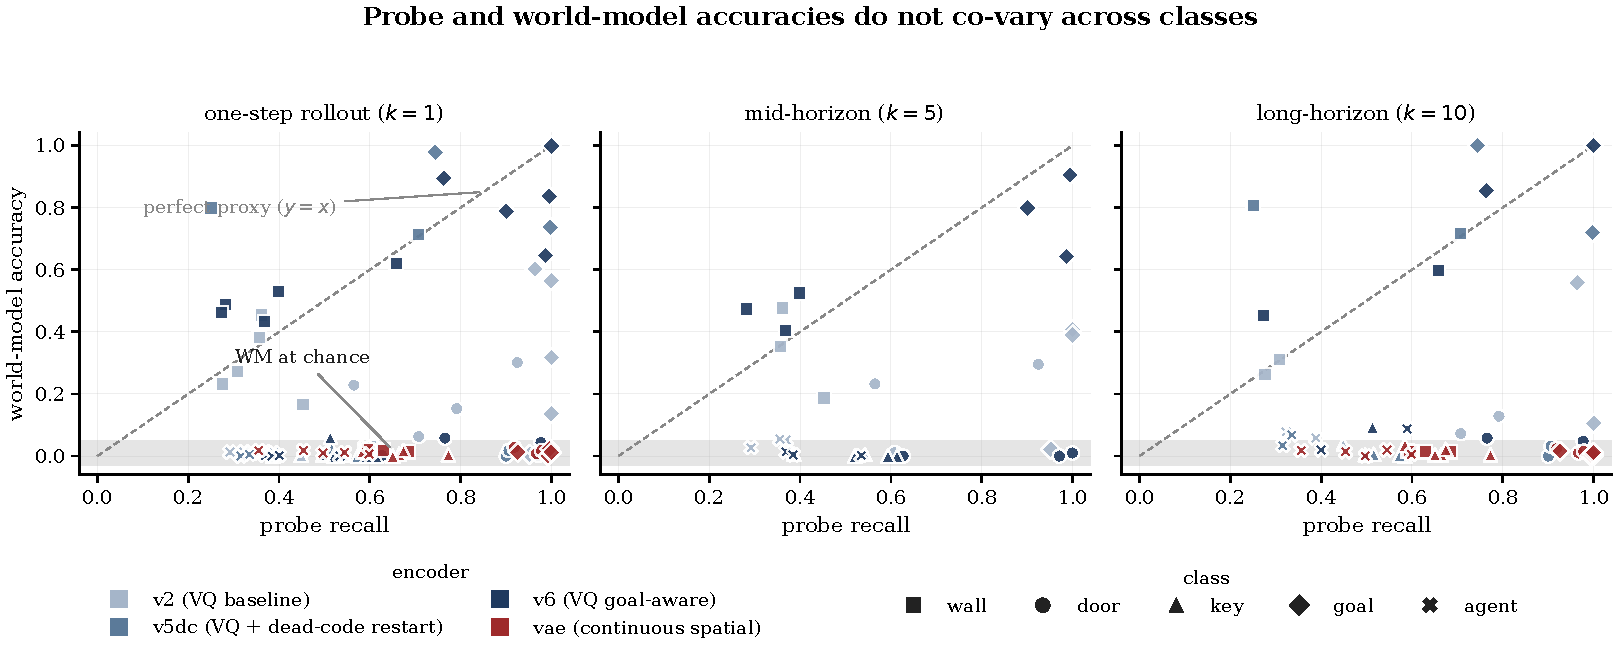
\includegraphics[width=0.95\linewidth]{fig1_probe_vs_wm_scatter.pdf}
  \caption{\textbf{Probe vs.\ WM scatter on DK-8.} Under the proxy null, points would follow $y{=}x$; instead most lie at WM$_k\!\approx\!0$ regardless of probe value, especially for \texttt{door}, \texttt{key}, and \texttt{agent}.}
  \label{fig:scatter}
\end{figure}

\begin{figure}[t]
  \centering
  \includeartifactfigure{width=0.95\linewidth}{fig8_oracle_gap_closure.pdf}
  \caption{\textbf{Offline oracle WM closes the probe-WM gap.} On the same frozen encoder and MLP architecture, oracle-WM accuracy matches or exceeds probe accuracy in $8$ of $9$ family--class aggregates.}
  \label{fig:oracle-gap}
\end{figure}

\paragraph{The gap responds to training procedure: an offline oracle WM closes most of it.}\label{sec:oracle}
We freeze the encoder, collect a $30{,}000$-transition buffer, and train the same MLP transition model offline-to-convergence. Across $10$ source checkpoints, pooled WM$_1$ rises from $0.02$ to $\mathbf{0.91}$ on \texttt{door}, $0.01\to\mathbf{0.88}$ on \texttt{key}, and $0.01\to\mathbf{0.81}$ on \texttt{agent} (Fig.~\ref{fig:oracle-gap}); per-family gap closure exceeds $97\%$ on all $9$ family--class aggregates. The random-only-buffer control closes the gap at least as well as the mixed policy buffer, and teacher-forcing at $k{=}10$ stays within $0.01$ of free-running on the rare classes, ruling out distribution mismatch and compounding error (Appendices~\ref{app:ablations}, \ref{app:planning-extra}). \textbf{The encoder carries the semantic information probes report, but this does not imply action-conditioned planning usability.}

This result calibrates the negative claim. We are not saying that the encoder has discarded the door, key, or agent labels; the oracle WM can recover them. The failure is more specific: the representation can be semantically recoverable while presenting too little action-conditioned variation for the transition model and planner.

\subsection{Mechanism: semantically decodable latents can be action-blind}\label{sec:mechanism}

The oracle experiment of \S\ref{sec:oracle} shows that the encoder contains probe-recoverable semantic state information. However, semantic one-step predictability is not the same as action-identifiability: a latent can support class recovery while still collapsing the action-conditioned variation needed by a planner. We test this by directly probing the geometry of the learned transition model.

\paragraph{Joint-trained WMs are action-blind.} On the original online-trained WM with \srcVA, the action\_dep\_ratio is $\mathbf{0.0003}$ and effective action rank is $\mathbf{1.0/7}$: the transition model has effectively collapsed all actions into a single state-only prediction. Across $5$ WM training procedures applied to this encoder (online, offline-oracle, head-calibrated, multi-step state-loss, spatial ConvNet), every resulting WM has action\_dep\_ratio $\leq 0.022$: \textbf{within this cohort, changing the WM training recipe does not rescue the encoder's action-blindness}. By contrast, other source encoders preserve substantial action signal under the same measurement. The pattern therefore points to the encoder as the limiting factor in this cohort, rather than to the particular WM training recipe (Table~\ref{tab:action-cond-cohort}):

\begin{table*}[t]
  \centering
  \caption{Action-conditioning is encoder-determined: \srcVA{} is uniquely degenerate; other cohorts preserve action signal. Internal IDs and per-checkpoint values: Appendix~\ref{app:phaseN}.}
  \label{tab:action-cond-cohort}
  \small
  \setlength{\tabcolsep}{4pt}
  \begin{tabularx}{\textwidth}{@{}>{\raggedright\arraybackslash}X c c c L{0.15\textwidth}@{}}
    \toprule
    Cohort & Pooled action\_dep\_ratio & Eff.\ rank / max & $N$ & Regime \\
    \midrule
    \srcVA{} (5 WM trainings) & $0.014 \pm 0.008$ & $2.6 / 7$ & 5 & R1 (blind) \\
    \srcVB{}, \srcVC{} (oracle, conv, calib, multistep) & $0.59 \pm 0.30$ & $6.4 / 7$ & 7 & R2/R3 \\
    DK-8 VQ-VAE (\encVQRestart, \encVQGoal, oracle\_rigor variants) & $0.69 \pm 0.33$ & $4.7 / 7$ & 9 & mostly R2/R3 \\
    DK-16 VQ-VAE (\encVQRestart, \encVQGoal, cb1024) & $0.27 \pm 0.21$ & $4.4 / 7$ & 8 & \encVQRestart{} R1, \encVQGoal{} R2/R3 \\
    Crafter VQ-VAE (cross-env) & $0.34 \pm 0.05$ & $11.3 / 17$ & 8 & R4 (training-fragile) \\
    \bottomrule
  \end{tabularx}
\end{table*}

\paragraph{Causal test: the $\lambda$-sweep across $3$ source encoders.} We fine-tune the source encoder with an auxiliary action-prediction loss
\begin{equation}
  \mathcal{L}_{\text{act}}(\omega, \xi) \;=\; -\log P_\xi\!\left(a_t \,\big|\, z_t,\, z_{t+1}\right),
\end{equation}
where $P_\xi$ is a small action-decoder MLP. Total objective: $\mathcal{L}_{\text{recon}} + \beta \mathcal{L}_{\text{KL}} + \lambda \mathcal{L}_{\text{act}}$. We sweep $\lambda \in \{0, 0.5, 2.0, 10.0\}$ over $3$ source encoders (\srcVA{}, \srcVB{}, \srcVC{}); for each of the $12$ resulting fine-tuned encoders we train an oracle WM offline and re-run probe and action-conditioning evaluation.

This intervention targets the encoder, not the transition model: the action decoder sees $(z_t,z_{t+1})$ and forces latent displacements to retain enough information to recover $a_t$. If probe accuracy falls while action-dependence rises under this controlled objective change, the trade-off is not merely correlational variation across unrelated checkpoints.

\inputartifacttable{tab:phase-r-pareto}{Action-conditioning vs. probe-accuracy trade-off across the $\lambda$-sweep. Key numeric results are summarized in the surrounding text when the generated table file is unavailable.}{tables/phase_R_pareto.tex}

The trade-off appears as a sharp, consistent shift across all three sources. Raising $\lambda$ to $0.5$ produces a $20$--$160\times$ jump in $\mathrm{action\_dep\_ratio}$ and an $8$--$17$ absolute-percentage-point drop in probe accuracy. The action-dependence gain saturates by $\lambda{=}0.5$ in all three cases. \textbf{Per-encoder Pearson($\mathrm{probe\_avg}$, $\mathrm{action\_dep\_ratio}$) is $-0.97$ on \srcVA{} (R1 action-blind), $-0.94$ on \srcVB{} (R2 partial signal), and $-0.66$ on \srcVC{} (R3 high baseline); pooled across $N{=}12$ data points: $\mathbf{-0.674}$.} The smaller magnitude on \srcVC{} reflects its narrower dynamic range (already partially action-identifiable at $\lambda{=}0$), not a directional reversal.

\paragraph{Replication across architectures, tasks, and environments.} We extend the controlled $\lambda$-sweep to $15$ additional source encoders covering both architecture classes and three further environments. \textbf{DK-8 VQ-VAE} ($4$ encoders): two \encVQGoal{} seeds traverse cleanly (Pearson $-0.85$, $-0.86$); one \encVQRestart{} seed starts already at action\_dep $1.78$ and saturates ($+0.30$). \textbf{DK-8 \encSpatialVAE} extension to $5$ seeds: per-encoder Pearson $\{-0.97, -0.94, -0.66, -0.95, -0.81\}$, mean $-0.87$. \textbf{DK-16 cross-task} ($3$ \encVQGoal{} seeds): $\{-0.82, -0.33, -0.59\}$. \textbf{Crafter cross-environment} ($4$ encoders): mixed signal, with the strongest cohort at $-0.96$ and one outlier at $+0.62$ reflecting Crafter's $17$-action stochasticity. \textbf{LavaCrossing-S9N1 cross-environment} ($2$ encoders): $-0.91$ and $-0.93$. Combining everything: $N{=}\mathbf{72}$ across $\mathbf{18}$ source encoders, $4$ environments (DK-$8$, DK-$16$, Crafter, LavaCrossing), and $2$ architecture classes; \textbf{$14$ of $18$ encoders show clearly negative Pearson} ($<-0.5$); the $4$ saturating cases are precisely the encoders that begin already action-identifiable at $\lambda{=}0$. Pooled per-encoder Pearson: $\mathbf{-0.63}$. The mechanism is therefore not VAE-specific, not DK-specific, and not MiniGrid-specific---it concerns the encoder objective, not the architecture or task. Internal IDs and per-encoder data: Appendix~\ref{app:regimes-extra}.

\paragraph{Interpretation.} Standard MBRL objectives map semantically equivalent states to nearby latents, which probes reward. But this clustering can remove the action-conditioned variance needed for $T(z,a)\neq T(z,a')$: semantic decodability and action-identifiability occupy competing corners of the encoder objective. This also explains why an oracle WM can recover semantic labels without becoming useful for action ranking; the transition model can learn what class is present while still seeing almost no action-conditioned displacement in latent space.

\paragraph{Implications.} Semantic WM accuracy and action-identifiability must be measured separately: an oracle WM can close the per-class gap while remaining useless for action ranking if $T(z,a)$ barely varies with $a$. After fitting a lightweight transition probe or candidate WM, $\mathrm{action\_dep\_ratio}$ cheaply indicates whether WM-Dyna is in the right regime (\S\ref{sec:regimes}, \S\ref{sec:recipe}).

\subsection{Consequence: action-blind WMs are planning-incoherent}\label{sec:planning-ceiling}

\paragraph{Imagined returns are uncorrelated with actual returns.} For each working-policy checkpoint, we compare WM-imagined return $\hat G_0$ (rolled forward with the trained policy and bootstrapped by $V_\eta$) to realized return $G_0$. \textbf{Across $20$ DK-8 checkpoints, rank correlation at $K{=}10$ is $+0.007 \pm 0.154$, with $17/20$ checkpoints showing $|r| \leq 0.2$.} Per-encoder means lie in $[-0.09,+0.07]$; bias is calibratable, rank-noise is not. The failure is therefore not merely bad calibration of the imagined return scale. It is specifically a ranking failure: a planner can shift or rescale biased values, but cannot recover an action ordering from nearly independent imagined and realized returns.

\paragraph{Semantic one-step fixes do not close the planning gap.} Across $5$ WM training procedures and $13$ encoders, pooled Pearson($\hat G_0,G_0$) is $\mathbf{+0.075\pm0.087}$ at $K{=}1$ and $+0.057\pm0.071$ at $K{=}10$. Sweeping $K$ leaves the rank correlation flat, and the oracle WM that closes the semantic gap reaches $-0.085\pm0.180$. Multi-step state loss, head calibration, and value-aligned losses likewise fail to produce action rankings distinguishable from zero. \emph{Single-step semantic accuracy is necessary but not sufficient for planning coherence.}

\paragraph{The bound is the critic, not the WM.} The trained value function's own rank correlation with realized return is only $\mathbf{+0.118\pm0.124}$ on the same $13$ checkpoints, matching the WM-bootstrap ceiling within noise. This matters because a one-step imagined return is essentially $\hat r+\hat\gamma V_\eta(\hat z_1)$ when per-step prediction is good; it inherits the critic's ability to rank sparse-reward outcomes. On DoorKey, return ranking is task-bound by binary success variance, so per-step WM improvements cannot exceed that critic ceiling. WM usability must therefore be diagnosed by action-level signal, not return-level signal. Full data: Appendix~\ref{app:planning-extra}.

\subsection{Four regimes of WM failure}\label{sec:regimes}

The results support four WM-failure regimes indexed by encoder action-conditioning and task difficulty.

\begin{table*}[t]
  \centering
  \small
  \caption{\textbf{Regime taxonomy for WM-Dyna.} Action-conditioning, vanilla PPO performance, and WM-Dyna outcome identify four regimes.}
  \label{tab:regime-summary}
  \setlength{\tabcolsep}{6pt}
  \begin{tabularx}{\textwidth}{@{}L{0.18\textwidth}L{0.16\textwidth}L{0.24\textwidth}X@{}}
    \toprule
    Regime & Action-cond.\ & Vanilla PPO & WM-Dyna outcome \\
    \midrule
    \textbf{(R1)} \srcVA{} & $0.0003$ (blind) & $+0.519 \pm 0.05$ (struggles) & $\Delta = -0.03$ (no signal) \\
    \textbf{(R2)} \srcVB{} & $0.677$ (strong) & $+0.800 \pm 0.12$ (intermediate) & $\Delta = +0.09$ (modest help) \\
    \textbf{(R3)} \srcVC{} & $0.340$ (moderate) & $+0.997 \pm 0.001$ (solves) & $\Delta = -0.45$ (destroys learning) \\
    \textbf{(R4)} Crafter VQ-VAE & $0.34 \pm 0.05$ & varies by ckpt & WM accuracy unstable across ckpts \\
    \bottomrule
  \end{tabularx}
\end{table*}

\textbf{(R1) Action-blind}: WM has no signal; vanilla PPO $\approx$ oracle-Dyna. \textbf{(R2) Goldilocks}: action-identifiable encoder plus vanilla headroom; oracle-Dyna helps. \textbf{(R3) Easy-task}: vanilla already solves; Dyna injects low-return imagined samples and hurts, even at small imagine ratios. \textbf{(R4) Training-fragile}: action signal exists, but WM accuracy is unstable across checkpoints, so action-identifiability alone is not sufficient.

\paragraph{Regime diagnostic.} Action-conditioning separates (R1) from (R2)--(R4); vanilla-PPO ceiling separates (R2) from (R3); offline-WM accuracy separates (R2)/(R3) from (R4). DK-16 confirms the encoder-determined split: \encVQRestart{} seeds map to R1, while \encVQGoal{} seeds map to R2/R3 depending on the policy ceiling (Appendix~\ref{app:phaseN}). The taxonomy is descriptive on the $18$ encoders we tested rather than prospectively validated; we read the three instruments as a screening rule (cheap and consistent on this corpus) rather than a tested predictor on held-out runs.

\subsection{Constructive recipe: $\lambda$-finetuning rescues Dyna}\label{sec:recipe}

The mechanism of \S\ref{sec:mechanism} predicts that fixing encoder action-blindness should unlock WM-augmented Dyna. \textbf{Selection rule.} We deliberately select the most action-blind source encoder in our diagnostic ($\srcVA$, $\mathrm{action\_dep\_ratio} = 0.0003$, regime R1)---that is, the worst case where prior WM-Dyna recipes already failed. The recipe is informative precisely there: it must succeed on the encoder where the diagnostic is most adversarial. Cross-encoder generalization to less degenerate regimes is treated separately below. For each $\lambda \in \{0, 0.5, 2.0, 10.0\}$ we take the fine-tuned encoder, train an oracle WM offline, and run fresh PPO with and without WM-Dyna ($300$k env steps, $\mathrm{imagine\_ratio}{=}0.5$, $2$ seeds per condition).

\begin{table}[h]
  \centering
  \small
  \caption{\textbf{$\lambda$-finetuning rescues Dyna on \srcVA.} $\lambda{=}0.5$ yields $\mathbf{+0.29}$ over the same-encoder no-Dyna PPO control; larger $\lambda$ is unstable.}
  \label{tab:phase-T}
  \begin{tabular}{r r r r}
    \toprule
    $\lambda$ & no-Dyna PPO (mean) & oracle-Dyna (mean) & $\Delta$ \\
    \midrule
    $0.0$ (control) & $0.597$ ($0.513, 0.680$) & $0.565$ ($0.535, 0.594$) & $-0.03$ \\
    $0.5$           & $0.569$ ($0.445, 0.692$) & $\mathbf{0.862}$ ($0.905, 0.819$) & $\mathbf{+0.29}$ \\
    $2.0$           & $0.517$ ($0.326, 0.708$) & $0.273$ ($\mathbf{0.000}, 0.546$) & $-0.24$ \\
    $10.0$          & $0.587$ ($0.582, 0.592$) & $0.439$ ($0.878, \mathbf{0.000}$) & $-0.15$ \\
    \bottomrule
  \end{tabular}
\end{table}

\textbf{Three observations on \srcVA.} The $\lambda{=}0$ control reproduces the original no-effect Dyna comparison, so the fine-tuning pipeline itself is not adding an advantage. The sweet spot $\lambda{=}0.5$ matches the Pareto saturation point in \S\ref{sec:mechanism}: the same intervention that makes the encoder action-identifiable makes Dyna useful. At $\lambda\geq2$, oracle-Dyna is bimodally unstable, suggesting that pushing the auxiliary action loss too hard damages the reconstruction geometry that the offline WM must still model.

\paragraph{Caveat on the recipe.} The recipe combines two offline ingredients (encoder fine-tuning, then offline oracle-WM training) before the online Dyna stage. It is therefore a proof-of-concept that fixing encoder action-identifiability \emph{can} unlock WM-Dyna, not a fully-online MBRL recipe; integrating $\lambda$-finetuning into joint online training is left to future work and noted in the limitations.

\paragraph{Cross-encoder generalization: the optimal $\lambda$ is regime-conditional.} We also ran the recipe on \srcVB{} (R2) and \srcVC{} (R3), $32$ runs total. Headline $\Delta$(oracle-Dyna $-$ no-Dyna PPO) at the per-encoder optimal $\lambda$:
\begin{table}[t]
  \centering
  \footnotesize
  \caption{\textbf{Regime-conditional $\lambda$ transfer across source encoders.} The constructive recipe helps only in regimes with headroom and an appropriate level of action-identifiability.}
  \label{tab:lambda-regime-transfer}
  \setlength{\tabcolsep}{2pt}
  \renewcommand{\arraystretch}{1.05}
  \begin{tabularx}{\linewidth}{@{}L{0.15\linewidth}L{0.20\linewidth}cL{0.23\linewidth}X@{}}
    \toprule
    Source encoder & Regime & Optimal $\lambda$ & $\Delta$ at optimum (per-seed Dyna returns) & Failure modes \\
    \midrule
    \srcVA{} & R1 (action-blind) & $\mathbf{0.5}$ & $\mathbf{+0.29}$ ($0.905, 0.819$) & $\lambda\geq 2$: bimodal collapse \\
    \srcVB{} & R2 (partial action-identifiable) & $\mathbf{2.0}$ & $\mathbf{+0.15}$ ($0.932, 0.918$) & $\lambda{\in}\{0.5, 10\}$: one-seed collapse \\
    \srcVC{} & R3 (vanilla solves) & none & none ($\lambda{=}0.5$ collapses $\to 0.0$) & every $\lambda$ underperforms vanilla \\
    \bottomrule
  \end{tabularx}
\end{table}
The optimal $\lambda$ shifts with the starting regime: $\lambda{=}0.5$ rescues R1, $\lambda{=}2.0$ helps R2, and every $\lambda$ hurts R3. Thus the prescription is regime-conditional in our setting: measure $\mathrm{action\_dep\_ratio}$ first; use $\lambda{=}0.5$ for R1, $\lambda{=}2.0$ for R2, and no Dyna for R3. The same $\lambda$ that repairs an action-blind encoder can destroy an already-solving encoder, which is why the diagnostic must precede the recipe. Full sweeps: Appendix~\ref{app:regimes-extra}.

We view this as constructive evidence, not a definitive performance benchmark: each Dyna cell has two seeds, and the instability at high $\lambda$ is itself part of the finding. The important point is that the intervention predicted by the mechanism changes a previously useless WM recipe into a beneficial one in the regime where it should.

\section{Discussion and Conclusion}

Probe accuracy is not a certificate of WM usability. Under our intervention, semantic decodability trades off against action-identifiability: $\mathrm{action\_dep\_ratio}$ rises $20$--$160\times$ while probe accuracy drops $8$--$17$ pp across $3$ source encoders, with pooled Pearson $-0.67$ (\S\ref{sec:mechanism}). The constructive result is regime-bounded: $\lambda{=}0.5$ transforms a useless WM-Dyna recipe into a $+0.29$ return improvement over the same-encoder no-Dyna control in R1, while stronger or unnecessary regularization can hurt.

\paragraph{Recommendations.} Report semantic probe accuracy alongside action-identifiability and offline-WM accuracy. Before expensive Dyna rollouts, fit a lightweight transition probe or candidate WM and measure \S\ref{sec:mechanism}'s diagnostic. In the regimes we observe, the resulting recipe is specific: R1 fine-tune at $\lambda{=}0.5$, R2 at $\lambda{=}2.0$, R3 avoid Dyna, and R4 check offline-WM accuracy first. The mechanism is at the encoder-action-conditioning level, so the encoder objective itself may need to be modified rather than relying on transition-model training alone. This keeps probes in the evaluation stack, but demotes them from certificates to one diagnostic among several. Practically, this changes the reporting standard: a high-probe model should be accompanied by evidence that actions remain identifiable in the latent dynamics.

\paragraph{Limitations.} We test $4$ environments (DK-$8$, DK-$16$, Crafter, LavaCrossing) with linear probes, MLP/spatial-Conv transitions, and $N{=}72$ causal sweep cells across $18$ source encoders spanning $2$ architecture classes; $14$ of $18$ per-encoder Pearson values are $< -0.5$, and the $4$ saturating cases all start already action-identifiable. The diagnostic is sufficient but not necessary: R4 shows action-identifiable encoders can still produce unstable WMs, so offline-WM accuracy remains necessary. Richer probes, RSSMs, Transformers, diffusion dynamics, object-centric encoders, and end-to-end PPO fine-tuning may shift the trade-off. The present claim is therefore calibrated: probe accuracy alone can be misleading and, under this intervention, anti-aligned with action-identifiability; it is not a universal claim that all probes are harmful. Future work should test whether action-identifiability can be built into pretraining rather than repaired post hoc, and whether adaptive $\lambda$ schedules can avoid the high-dose instability we observe. Extended limitations and impact are in Appendices~\ref{app:limitations}, \ref{app:impact}.

\bibliographystyle{plainnat}
\bibliography{ref}

\newpage
\appendix

\section{Architecture and training objective --- full details}\label{app:arch-detail}

\paragraph{What each module consumes.}
The three consumers do not all see the same object:
\begin{table}[h]
  \centering
  \caption{Inputs consumed by probes, policy/value heads, and transition models for VQ and VAE encoders.}
  \label{tab:module-consumers}
  \begin{tabular}{l l l}
    \toprule
    Consumer & VQ input & VAE input \\
    \midrule
    Probe & $\tilde\phi(o_t)$ (continuous $D$-dim per cell) & $\mu(o_t)$ (continuous $D$-dim per cell) \\
    Policy / value & $\mathrm{vec}(\tilde\phi(o_t))$ (continuous, STE) & $\mathrm{vec}(\mu(o_t))$ (continuous) \\
    WM $f_\theta$ (main loss) & code indices $z_t$ (via internal embed.) & $\mathrm{vec}(\mu(o_t))$ (continuous) \\
    WM aux loss $\mathcal{L}_{\text{aux}}$ & $\mathrm{vec}(\tilde\phi(o_t))$ (continuous, STE) & (disabled) \\
    \bottomrule
  \end{tabular}
\end{table}

\paragraph{Joint training objective.}
\begin{equation}
  \mathcal{L}(\omega, \psi, \theta, \eta) = \mathcal{L}_{\text{PPO}}(\eta) + \lambda_{\text{rec}} \mathcal{L}_{\text{rec}}(\omega, \psi) + \lambda_{\text{wm}} \mathcal{L}_{\text{wm}}(\omega, \theta) + \alpha_{\text{aux}} \mathcal{L}_{\text{aux}}(\omega, \psi, \theta) + \lambda_{\text{sem}} \mathcal{L}_{\text{sem}}(\omega, \psi).
\end{equation}
$\mathcal{L}_{\text{rec}}$ is pixel MSE (plus KL for the VAE). $\mathcal{L}_{\text{wm}}$ is the transition trainer's online one-step loss on a FIFO transition buffer: cross-entropy on $z_{t+1}$ given code indices $z_t$ for VQ; feature MSE on $\mu(o_{t+1})$ given the continuous latent for the VAE. $\mathcal{L}_{\text{aux}}$ is a PPO-batch cross-entropy on $z_{t+1}$ predicted by $f_\theta$ from $(\mathrm{vec}(\tilde\phi(o_t)), a_t)$, undefined for continuous codes (so $\alpha_{\text{aux}}{=}0$ for the VAE). Where enabled, $\mathcal{L}_{\text{sem}}$ is the 11-class semantic auxiliary described below; otherwise $\lambda_{\text{sem}}{=}0$. All four modules are trained jointly and on-policy; the world model is not trained to convergence on a fixed dataset but on a sliding buffer of actual transitions emitted by the current policy. This is the standard learned-latent MBRL training loop \citep{hafner2019dream,micheli2023iris,alonso2024diamond}.

\paragraph{Probe formulation.}
We fit one shared logistic regression across all token positions, $p_\beta(c \mid \tilde\phi(o)_{:,i,j}) \propto \exp(\beta_c^\top \tilde\phi(o)_{:,i,j})$, using scikit-learn with class-balanced weights ($N/(|\mathcal{C}|\, n_c)$), $C{=}1.0$, max 300 iterations. Per-class probe accuracy is recall: the count of cells with both true and predicted class $c$, divided by the count with true class $c$.

\section{Hyperparameters and reproducibility}\label{app:hparams}

\paragraph{Experimental grid.} Main text uses descriptive encoder names; the internal IDs are the artifact and log names used in released files. $K$ = VQ codebook size; \emph{D.C.} = dead-code restart; \emph{Quant.} = quantization bottleneck; S = seed count.
\begin{table}[h]
  \centering
  \caption{Joint-trained checkpoint grid for \S\ref{sec:correlation}, with paper-facing condition names mapped to internal artifact IDs. $^\star$All three DK-16 \encVQRestart{} seeds collapsed to a near-empty effective codebook and are excluded from the pooled correlation (Appendix~\ref{app:dk16-v5dc}).}
  \label{tab:exp-grid}
  \resizebox{\linewidth}{!}{%
    \begin{tabular}{l l l c c c c c}
      \toprule
      Env & Paper name & Internal ID & $K$ & D.C. & Quant. & $\alpha_{\text{aux}}$ & S \\
      \midrule
      DK-8  & \encVQBase      & \texttt{v2}   & 64  &      & $\checkmark$ & 0.1 & 5 \\
      DK-8  & \encVQNoRestart & \texttt{v5}   & 64  &      & $\checkmark$ & 0.1 & 3 \\
      DK-8  & \encVQRestart   & \texttt{v5dc} & 64  & $\checkmark$ & $\checkmark$ & 0.1 & 2 \\
      DK-8  & \encVQGoal      & \texttt{v6}   & 64  &      & $\checkmark$ & 0.1 & 5 \\
      DK-8  & \encVQWide      & \texttt{v9}   & 64  &      & $\checkmark$ & 0.1 & 3 \\
      DK-8  & \encSpatialVAE  & \texttt{vae}  & --- & ---  &              & 0.0 & 5 \\
      DK-16 & \encVQGoal      & \texttt{v6}   & 512 &      & $\checkmark$ & 0.1 & 3 \\
      DK-16 & \encVQRestart   & \texttt{v5dc} & 512 & $\checkmark$ & $\checkmark$ & 0.1 & 3$^\star$ \\
      \bottomrule
    \end{tabular}
  }
\end{table}

\paragraph{Encoder backbone.}
All encoders share a 4-layer convolutional backbone with channel widths $(32, 64, 128, D{=}64)$, stride-2 downsampling at each layer, and ReLU activations. The filter size at the first layer is $9$ for \encVQBase{} and $8$ for the other DK encoder families. Decoders are the symmetric transpose-convolutional inverse of the encoder. The VQ codebook size is $K{=}64$ for DK-8 and $K{=}512$ for DK-16; codebook vectors are 64-dim and trained with the EMA update of \citet{razavi2019vqvae2} with decay 0.99. Dead-code restart (\encVQRestart) re-initializes any code with usage count below $\tau{=}2.0$ in the most recent transition buffer window.

\paragraph{World-model MLP.}
Hidden width 256, depth 3, ReLU, layer-norm. Action embedding 32-dim. For VQ encoders, code indices are first embedded ($K \to 64$) before being flattened and concatenated with action embedding; the output head produces $H'W' \times K$ logits decoded by argmax. For the VAE, the input and output are flat continuous vectors of dimension $D \cdot H' \cdot W'$. Same architecture across all encoder families.

\paragraph{PPO training.}
We use the standard PPO actor-critic with a single-network shared backbone (the encoder) and small policy/value heads (2-layer MLPs of width 64). Hyperparameters: 16 parallel environments, 4096-transition rollout buffer per update, 10 inner epochs, minibatch size 64, clip ratio $0.2$, entropy coefficient $0.01$, GAE $\lambda{=}0.95$, discount $\gamma{=}0.99$, learning rate $1{\times}10^{-4}$ (cosine-annealed to $0$ over training), max gradient norm $0.5$, value-function clipping enabled, normalized advantages.

\paragraph{Encoder learning rate.}
The encoder is trained with a separate learning rate $1{\times}10^{-5}$, also cosine-annealed, with a \emph{snap-back} regularizer: when the rolling-window mean reward drops by more than $0.5$ relative to its best, the encoder learning rate is briefly reset to its initial value for $100$ updates. This prevents the encoder from collapsing during PPO instability.

\paragraph{Auxiliary losses.}
Reconstruction weight $\lambda_{\text{rec}}{=}1.0$ (pixel MSE plus VQ commitment $\lambda_{\text{commit}}{=}0.25$, or VAE $\beta{=}1.0$). World-model auxiliary $\alpha_{\text{aux}}{=}0.1$ for VQ encoders, $0$ for the VAE. Where enabled, the semantic auxiliary uses $\lambda_{\text{sem}}{=}0.05$ on an 11-class classification head reading from the post-bottleneck features (focal loss with $\gamma{=}2$, class-balanced weights, hidden 128). The transition trainer runs $\mathcal{L}_{\text{wm}}$ on a FIFO buffer of the most recent $10^5$ transitions with batch size $256$.

\paragraph{Training budget.}
DK-8: 5M environment steps per run, $\approx 2$ hours on a single NVIDIA RTX 4090. DK-16: 8M environment steps, $\approx 9$ hours. Analysis (probe fit + 500 free-running rollouts at 4 horizons) runs in $\sim$2 minutes per checkpoint.

\paragraph{Ground-truth class extraction.}
MiniGrid frames carry an underlying object grid with integer object IDs ($\texttt{empty}{=}1$, $\texttt{wall}{=}2$, $\texttt{door}{=}4$, $\texttt{key}{=}5$, $\texttt{goal}{=}8$, $\texttt{agent}{=}10$, plus state-conditional codes). We extract this grid via the \texttt{grid.encode()} method of the underlying \texttt{minigrid.MiniGridEnv}; this label is used for the probe and per-class WM evaluation, and for the semantic auxiliary in variants that explicitly enable that head. It is not used by the transition trainer, policy/value objective, Dyna rollouts, or planning-coherence metrics.

\paragraph{Software and seeds.}
PyTorch 2.1, gymnasium $0.29$, MiniGrid $2.3$, scikit-learn $1.3$. All randomness (env, model init, action sampling, dataloader) is seeded with the run seed. Code at \texttt{[anonymized URL]}; per-checkpoint analysis JSONs and the script that produced every figure in this paper (\texttt{paper\_assets/make\_figures.py}) are released alongside.

\section{Probe evaluation protocol --- full details}\label{app:probe-protocol}

We do not hold out a test split. Linear probes with $O(10^3)$ parameters on $O(10^6)$ samples are far from overfitting in the generalization-gap sense, so the training-set recall is within a few percentage points of a held-out recall on this data; but the reported number is nonetheless an upper bound on probe generalization. If the probe were hand-tuned downward by a held-out split, the gap between Probe$_c$ and WM$_c^{(k)}$ would only widen.

The buffer is drawn from random actions, which biases it toward states near episode start (agent exploring near the spawn) and away from states that require key pickup to reach. This makes \texttt{door}, \texttt{key}, and \texttt{goal} instances rarer in the buffer than under the trained policy, but not absent: the 16-env parallel walk at horizon $\approx 50$ still exposes doors and keys in every episode. The WM evaluation uses the same random-action distribution, so the probe and the WM are measured on matched states.

Recall (rather than precision or $F_1$) is reported because the dissociation we study concerns \emph{retrieving} task-critical classes from the latent, and recall is the most direct per-class measure of this.

\section{World-model accuracy protocol --- full details}\label{app:wm-protocol}

\paragraph{Bucketing alternative.}
An alternative metric that buckets cells by class at step $k$ rather than at $t{=}0$ is reasonable too, but conflates the WM's ability to track existing class-$c$ cells with its ability to \emph{generate new} class-$c$ cells (e.g.\ a door disappearing or an agent teleporting into a position). We avoid that conflation and bucket by the ground-truth class at $t{=}0$ (\texttt{sem\_labels\_0} in \texttt{analyze\_wm\_multistep.py:273}).

\paragraph{Free-running rollout under random actions.}
We feed the WM's own output back as input at every step and use the same random-action policy that generated the probe buffer. This matches the conditions under which a planner would query the WM and uses the same state distribution as the probe.

\paragraph{Per-cell match, not feature MSE.}
For \encSpatialVAE{}, the WM's output is a real-valued vector. We use a \textbf{cosine-similarity argmax within a frame}: a predicted token at position $(i,j)$ is correct iff, among all $H'W'$ tokens in the same frame, the one whose normalized embedding has the highest cosine similarity to $\hat\ell_{k, ij}$ is the one at position $(i, j)$ in the true encoding. This avoids introducing a post-hoc quantizer (a free parameter that would bias the comparison) and is strictly stronger than continuous MSE.

\section{Spatial-VAE architecture and loss}\label{app:vae-spatial}

Given the encoder output $\phi_\omega(o) \in \mathbb{R}^{D \times H' \times W'}$, \texttt{AEModelSpatial} applies two $1 \times 1$ convolutions:
\begin{equation}
  \mu(o) = \mathrm{Conv}_{1\times 1}^\mu\big(\phi_\omega(o)\big), \qquad
  \log\sigma(o) = \mathrm{Conv}_{1\times 1}^\sigma\big(\phi_\omega(o)\big), \qquad
  \mu, \log\sigma \in \mathbb{R}^{D \times H' \times W'}.
\end{equation}
The latent is $z(o) = \mu(o) + \sigma(o) \odot \epsilon$ with $\epsilon \sim \mathcal{N}(0, I)$; at inference we use $\mu$. For use by the flat MLP transition model and the PPO policy head, $z$ is flattened to $\mathbb{R}^{D \cdot H' \cdot W'}$; the original spatial structure is recovered by reshape whenever per-cell access is needed.

\texttt{AEModelSpatial} is trained under a standard $\beta$-VAE objective
\begin{equation}
  \mathcal{L}_{\text{rec}}(\omega, \psi) = \mathbb{E}_{z \sim q_\omega}[\|\mathrm{dec}(z) - o\|^2] + \beta \cdot D_{\text{KL}}\big(q_\omega(z \mid o) \,\|\, \mathcal{N}(0, I)\big),
\end{equation}
with $\beta$ matched to the default VQ commitment coefficient. The decoder, policy head, and transition MLP are otherwise identical to \encVQGoal.

The continuous-latent scoring rule applies the cosine-similarity argmax within a frame directly to the per-cell slices of the flat latent, with no auxiliary codebook. This keeps the evaluation protocol as close as possible to the VQ case.

\section{Full per-class results}\label{app:full-tables}

\subsection{\encSpatialVAE{} full per-class table (5 seeds)}

\begin{table}[h]
  \centering
  \caption{Full per-class table for the \encSpatialVAE{} comparison (5 seeds).}
  \label{tab:full-vae}
  \begin{tabular}{l c c c}
    \toprule
    Class & Probe & WM$_1$ & WM$_{10}$ \\
    \midrule
    wall  & $0.620\pm0.044$ & $0.017\pm0.008$ & $0.015\pm0.001$ \\
    door  & $0.970\pm0.028$ & $0.008\pm0.007$ & $0.009\pm0.007$ \\
    key   & $0.669\pm0.062$ & $0.016\pm0.008$ & $0.014\pm0.008$ \\
    goal  & $0.983\pm0.028$ & $0.012\pm0.009$ & $0.006\pm0.005$ \\
    agent & $0.500\pm0.070$ & $0.015\pm0.005$ & $0.013\pm0.008$ \\
    \bottomrule
  \end{tabular}
\end{table}

\subsection{DoorKey-16$\times$16: full per-class table (\encVQGoal, 3 seeds)}\label{app:dk16-table}

\begin{table}[h]
  \centering
  \caption{DoorKey-16$\times$16 \encVQGoal{} per-class probe vs.\ 1-step world-model accuracy (3 seeds). The probe tightens at DK-16 while the WM gap widens on \texttt{door}, \texttt{key}, and \texttt{agent}.}
  \label{tab:dk16-v6-table}
  \begin{tabular}{l c c}
    \toprule
    Class & Probe & WM$_1$ \\
    \midrule
    wall  & $0.662\pm0.022$ & $0.599\pm0.015$ \\
    door  & $1.000\pm0.000$ & $0.045\pm0.028$ \\
    key   & $0.958\pm0.034$ & $0.115\pm0.085$ \\
    goal  & $1.000\pm0.000$ & $0.995\pm0.007$ \\
    agent & $0.591\pm0.081$ & $0.074\pm0.047$ \\
    \bottomrule
  \end{tabular}
\end{table}

\subsection{DK-8 vs.\ DK-16 side-by-side bar plot (\encVQGoal)}

\begin{figure}[h]
  \centering
  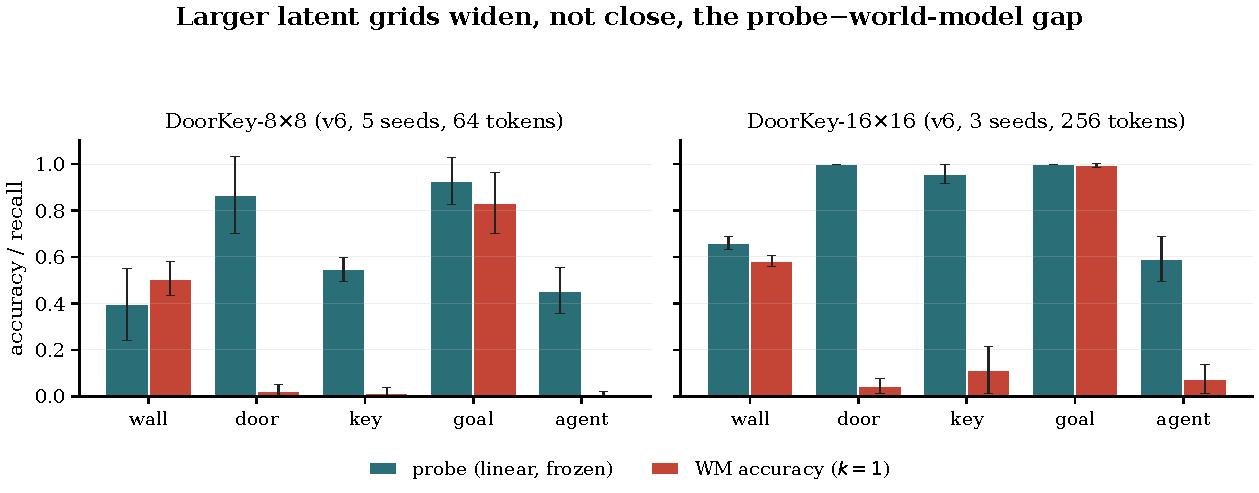
\includegraphics[width=0.95\linewidth]{fig4_dk8_vs_dk16.pdf}
  \caption{\textbf{The probe--WM gap replicates and widens at larger latent grids.} Per-class probe recall (teal) and WM$_1$ (red) for \encVQGoal{} on DoorKey-8$\times$8 (left, 5 seeds, 64 tokens) and DoorKey-16$\times$16 (right, 3 seeds, 256 tokens). Moving to the larger grid tightens the probe on \texttt{door}, \texttt{key}, \texttt{goal} (all $\ge 0.96$) while WM accuracy on \texttt{door}, \texttt{key}, \texttt{agent} stays $\le 0.12$.}
  \label{fig:dk8_vs_dk16}
\end{figure}

\subsection{Dead-code restart vs.\ no-restart side-by-side (\encVQNoRestart{} vs.\ \encVQRestart)}

\begin{figure}[h]
  \centering
  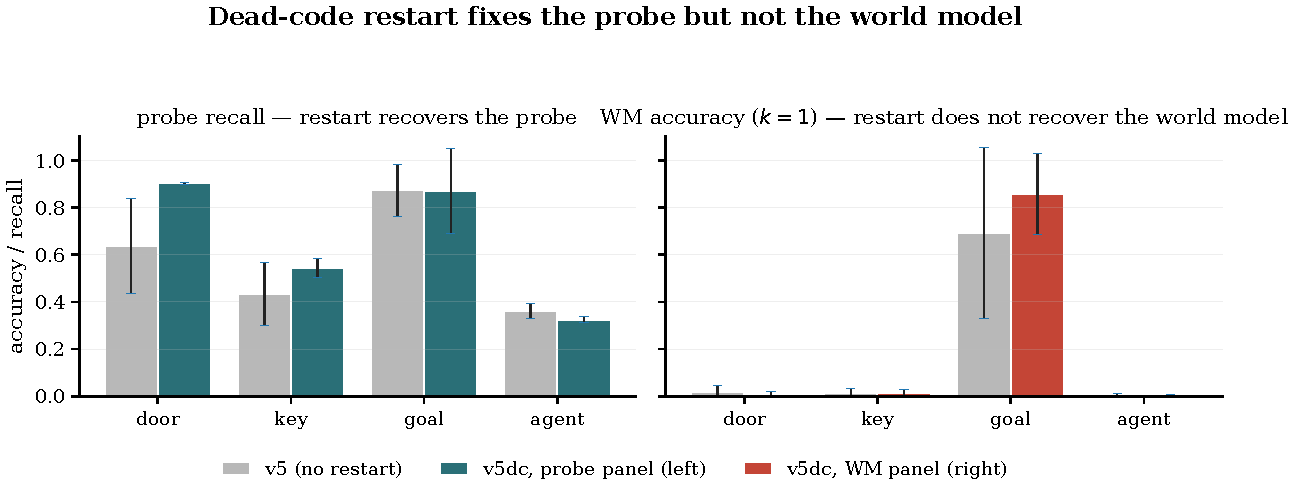
\includegraphics[width=0.92\linewidth]{fig5_deadcode_dissociation.pdf}
  \caption{\textbf{Dead-code restart recovers the probe but not the world model (DK-8).} Left: probe recall. Adding dead-code restart (\encVQRestart, teal) to the \encVQNoRestart{} baseline (gray) raises probe recall on \texttt{door} from $0.63$ to $0.90$ and on \texttt{key} from $0.43$ to $0.54$. Right: WM$_1$ accuracy stays at the floor ($\le 0.02$) on \texttt{door}, \texttt{key}, and \texttt{agent} for both encoders. The \texttt{goal} column is high on both bars in the right panel, consistent with the goal's spatial stationarity. Error bars are $\pm$std (\encVQNoRestart: 3 seeds; \encVQRestart: 2 seeds).}
  \label{fig:deadcode}
\end{figure}

\subsection{Auxiliary VQ encoder controls (\encVQNoRestart, \encVQWide; DK-8)}\label{app:v5-v9}

The pooled correlation in Table~\ref{tab:pearson-extended} draws on the four headline families plus two auxiliary VQ controls: \textbf{\encVQNoRestart} (the no-restart VQ baseline) and \textbf{\encVQWide} (a wider VQ variant). Both are reprobed from earlier checkpoints with the same protocol as the main runs. Per-encoder seed counts in the 100-checkpoint pool are reported in Table~\ref{tab:pearson-per-encoder-extended}.

\inputartifacttable{tab:pearson-extended}{Pooled across-class Pearson correlations under exact and apples-to-apples world-model scoring rules.}{tables/pearson_pooled_extended.tex}

\inputartifacttable{tab:pearson-per-encoder-extended}{Per-encoder across-class Pearson correlations under exact and apples-to-apples world-model scoring rules.}{tables/pearson_per_encoder_extended.tex}

\begin{table}[h]
  \centering
  \caption{\encVQNoRestart{} (no-restart VQ baseline, 3 seeds) and \encVQWide{} (wider VQ variant, 3 seeds) per-class probe and WM accuracy on DK-8. Same dissociation pattern as the main families: probes recover task objects while WM$_1$ stays near the floor for position-varying classes.}
  \label{tab:v5-v9}
  \begin{tabular}{l c c c c c}
    \toprule
    Class & Probe (\encVQNoRestart) & WM$_1$ (\encVQNoRestart) & Probe (\encVQWide) & WM$_1$ (\encVQWide) & WM$_5$ (\encVQWide) \\
    \midrule
    wall  & $0.276\pm0.122$ & $0.684\pm0.017$ & $0.389\pm0.072$ & $0.390\pm0.064$ & $0.381\pm0.028$ \\
    door  & $0.638\pm0.165$ & $0.017\pm0.023$ & $0.866\pm0.091$ & $0.007\pm0.008$ & $0.003\pm0.004$ \\
    key   & $0.434\pm0.109$ & $0.013\pm0.017$ & $0.617\pm0.063$ & $0.001\pm0.002$ & $0.000\pm0.000$ \\
    goal  & $0.873\pm0.091$ & $0.691\pm0.296$ & $0.982\pm0.003$ & $0.607\pm0.411$ & $0.613\pm0.425$ \\
    agent & $0.362\pm0.026$ & $0.006\pm0.004$ & $0.502\pm0.017$ & $0.003\pm0.002$ & $0.005\pm0.001$ \\
    \bottomrule
  \end{tabular}
\end{table}

\subsection{DK-16 \encVQRestart{} codebook collapse: full per-class table}\label{app:dk16-v5dc}

\begin{table}[h]
  \centering
  \caption{DK-16 \encVQRestart{} per-class probe and WM accuracy (3 seeds). Probe recall is at or near chance on task-critical classes, reflecting near-empty effective codebook utilization at $K{=}512$.}
  \label{tab:dk16-v5dc-table}
  \begin{tabular}{l c c c}
    \toprule
    Class & Probe & WM$_1$ & WM$_{10}$ \\
    \midrule
    wall  & $0.052\pm0.017$ & $0.035\pm0.027$ & $0.023\pm0.010$ \\
    door  & $0.266\pm0.147$ & $0.009\pm0.009$ & $0.013\pm0.009$ \\
    key   & $0.473\pm0.353$ & $0.019\pm0.009$ & $0.015\pm0.014$ \\
    goal  & $0.661\pm0.388$ & $0.333\pm0.470$ & $0.333\pm0.470$ \\
    agent & $0.127\pm0.041$ & $0.002\pm0.002$ & $0.013\pm0.003$ \\
    \bottomrule
  \end{tabular}
\end{table}

\section{Planning-coherence details}\label{app:planning-extra}

\paragraph{Original $20$-checkpoint planning rank correlation.} For each working-policy checkpoint we run $100$ trained-policy episodes in the env, then for each starting state run the WM forward $K$ steps using the policy's chosen actions and accumulate $\hat G_0 = \sum_{k} (\prod_{j<k} \hat\gamma_j) \hat r_k + (\prod \hat\gamma) V_\eta(\hat z_K)$. We compare $\hat G_0$ to the actual discounted return $G_0 = \sum_t \gamma^t r_t$. Across $20$ working-policy DK-8 checkpoints spanning six encoder families, the rank correlation between $\hat G_0$ and $G_0$ at $K{=}10$ is $+0.007 \pm 0.154$, with $17/20$ checkpoints showing $|r| \leq 0.2$. Per-encoder means lie in $[-0.09, +0.07]$. The trained value head applied to the true initial state $z^\star_0$ is well-calibrated ($\bar V(z^\star_0) \approx \bar G_{\text{real}}$ to within $0.05$); the dysfunction is specific to the WM-rolled imagined return, not to the value head itself. Bias direction varies wildly by family (\encSpatialVAE{} $\bar{\hat G}_0 - \bar G_0 \approx -0.5$; \encVQRestart{} $\approx -1.7$; \encVQNoRestart{} $\approx -7.3$); bias is calibratable, rank-noise is not.

\inputartifacttable{tab:planning-rank}{Rank correlation between imagined and realized returns across working-policy checkpoints. Key numeric results are summarized in the surrounding text when the generated table file is unavailable.}{tables/planning_rank_correlation.tex}

\paragraph{Five WM training procedures, full data.} The $13$-checkpoint corpus underlying \S\ref{sec:planning-ceiling} spans: original online joint-trained WM, offline-oracle WM, head-calibrated variant, multi-step state-loss variant ($K{=}5$ teacher-free), and value-aligned variant (frozen-critic auxiliary along the imagined trajectory). Across all $13$, pooled imagined-vs-real rank correlation is $+0.075 \pm 0.087$ at $K{=}1$ and $+0.057 \pm 0.071$ at $K{=}10$. Per-cohort means at $K{=}1$ lie in $[+0.03, +0.15]$. Sweeping $K \in \{1, 2, 3, 5, 7, 10\}$ shows the rank correlation is essentially flat with $K$, ruling out compounding error.

\paragraph{Oracle WM does not fix planning incoherence.} On the oracle ckpts of \S\ref{sec:oracle}, pooled rank correlation at $K{=}10$ is $-0.085\pm0.180$ (mixed buffer, $N{=}8$); per-encoder the oracle does not improve over the online WM (\encVQGoal{} oracle: $-0.16\pm0.18$ on $5$ ckpts vs.\ online $+0.06\pm0.18$). Single-step accuracy is therefore necessary but not sufficient for planning coherence.

\paragraph{Downstream-usability check (E8).} On $13$ checkpoints we load the trained PPO policy $\pi_\eta$ and value head $V_\eta$, roll the policy in the env (50 episodes), free-run the WM from each visited state, and apply $\pi_\eta, V_\eta$ to both $z^\star_k$ and $\hat z_k$ at $k\in\{1,5,10\}$. On the informative DK-8 subset, action-match between $\arg\max\pi(z^\star_k)$ and $\arg\max\pi(\hat z_k)$ saturates at $0.29$--$0.44$ with KL median $1.0$--$4.8$~nats; value\_corr is near zero or negative ($-0.42\pm0.18$ at $k{=}1$ for DK-8 \encVQGoal{}). The disagreement is already saturated at $k{=}1$.

\inputartifacttable{tab:e8-coherence}{Policy/value coherence between true and world-model-imagined latents across horizons. Key numeric results are summarized in the surrounding text when the generated table file is unavailable.}{tables/e8_policy_value_coherence.tex}

\paragraph{Compounding error (teacher-forcing).} Teacher-forced and free-running WM accuracy at $k{=}10$ differ by less than $0.01$ on \texttt{door}, \texttt{key}, \texttt{agent} (e.g.\ \encVQGoal{} N=16: door $0.029 \to 0.032$; key $0.069 \to 0.078$; agent $0.053 \to 0.078$). The WM cannot predict these classes even given the true previous state, ruling out compounding error.

\section{Action-conditioning diagnostic: per-checkpoint breakdown}\label{app:phaseN}

\paragraph{Per-checkpoint $\mathrm{action\_dep\_ratio}$.} On the $12$ DK-8 checkpoints summarized in \S\ref{sec:mechanism}: \texttt{online\_vae\_s1} $=0.0003$, eff.\ rank $1.0/7$; \texttt{multistep\_vae\_s1} $=0.014$; \texttt{oracle\_vae\_s1} $=0.017$; \texttt{conv\_vae\_s1\_h64} $=0.018$; \texttt{calib\_vae\_s1} $=0.022$; \texttt{calib\_vae\_s2} $=0.799$, eff.\ rank $6.7$; \texttt{conv\_vae\_s2\_h64} $=1.094$, eff.\ rank $7.0$; \texttt{conv\_vae\_s3\_h64} $=0.929$; \texttt{oracle\_vae\_s2} $=0.677$; \texttt{multistep\_vae\_s2} $=0.181$; \texttt{multistep\_vae\_s3} $=0.112$; \texttt{oracle\_vae\_s3} $=0.340$. Across the $9$ DK-8 VQ-VAE checkpoints (Phase S; $5$ \encVQRestart{}/\encVQGoal{} online + $4$ offline-oracle/calib/rigor variants): min $0.16$, max $1.30$, pool $0.69 \pm 0.33$, eff.\ rank pool $4.7/7$. The $8$ Crafter checkpoints (Phase Q): pool $0.34 \pm 0.05$, eff.\ rank $11.3/17$. The DK-16 cohort ($8$ checkpoints): \encVQRestart{} seeds $\{0.008, 0.029, 0.033\}$; \encVQGoal{} family $\{0.27, 0.51, 0.37, 0.55\}$; \texttt{rigor\_cb512} $0.39$.

\paragraph{Reward and gamma head action-variance.} For most checkpoints the reward and gamma heads have effectively zero action variance ($r$\_var $< 10^{-4}$, $\gamma$\_var $< 10^{-5}$): the WM's predicted reward and discount depend only on the encoded state, not on the action. The few exceptions (e.g.\ \texttt{conv\_vae\_s2\_h64} with $r$\_var $=10^{-3}$) coincide with the encoders that show high action\_dep\_ratio.

\section{Regime taxonomy: per-checkpoint Dyna comparisons}\label{app:regimes-extra}

\paragraph{Phase O: Dyna by source encoder.} Per-seed and per-mode returns underlying the regime characterization of \S\ref{sec:regimes}: \textbf{\srcVA} (R1; internal \texttt{vae\_s1}) vanilla $\{0.568, 0.469\}$, oracle-Dyna $\{0.568, 0.406\}$, bootstrap-only $\{0.587, 0.493\}$. \textbf{\srcVB} (R2; internal \texttt{vae\_s2}) vanilla $\{0.681, 0.920\}$, oracle-Dyna $\{0.929, 0.843\}$, bootstrap-only $\{0.478, 0.639\}$. \textbf{\srcVC} (R3; internal \texttt{vae\_s3}) vanilla $\{0.998, 0.996\}$, oracle-Dyna $\{0.644, 0.443\}$, bootstrap-only $\{0.668, 0.664\}$. $\Delta$(oracle$-$vanilla) is $-0.03$ on R1 (no signal), $+0.09$ on R2 (modest help), $-0.45$ on R3 (destroys learning).

\paragraph{Phase O-light: dose-response on \srcVC{} (R3).} Sweeping $\mathrm{imagine\_ratio} \in \{0.05, 0.1, 0.2, 0.5\}$ at $\lambda{=}0$ on the easy-task encoder: $0.05$ gives $+0.721 \pm 0.002$ ($\Delta = -0.28$ vs.\ vanilla $+0.997$); $0.1$ gives $+0.684 \pm 0.061$; $0.2$ gives $+0.806 \pm 0.075$; $0.5$ gives $+0.653 \pm 0.229$. \emph{No safe dose}: even $r{=}0.05$ underperforms vanilla by $-28\%$ in mean return.

\paragraph{Phase V (cross-encoder Dyna recipe transfer): full per-seed numbers.} The $\lambda$-finetuning recipe of \S\ref{sec:recipe} applied to \srcVB{} and \srcVC{}: $32$ runs total ($2$ encoders $\times$ $4$ $\lambda$ $\times$ $2$ modes $\times$ $2$ seeds). Per-seed final returns (last $50$ episodes):

\begin{table}[h]
  \centering
  \small
  \caption{Full per-seed Phase V Dyna recipe transfer results for \srcVB{} and \srcVC{}.}
  \label{tab:phase-v-full}
  \begin{tabular}{l r r r r}
    \toprule
    Source & $\lambda$ & no-Dyna seeds (s1, s2) & oracle-Dyna seeds (s1, s2) & $\Delta$ \\
    \midrule
    \srcVB{} & $0.0$ & $0.532, 0.420$ & $0.523, 0.304$ & $-0.06$ \\
    & $0.5$ & $0.620, 0.421$ & $0.903, \mathbf{0.000}$ & $-0.07$ \\
    & $\mathbf{2.0}$ & $0.902, 0.649$ & $\mathbf{0.932, 0.918}$ & $\mathbf{+0.15}$ \\
    & $10.0$ & $0.993, 0.493$ & $0.924, \mathbf{0.000}$ & $-0.28$ \\
    \midrule
    \srcVC{} & $0.0$ & $0.557, 0.661$ & $0.471, 0.556$ & $-0.10$ \\
    & $0.5$ & $0.525, 0.998$ & $\mathbf{0.000, 0.000}$ & $-0.76$ \\
    & $2.0$ & $0.997, 0.998$ & $0.778, 0.930$ & $-0.14$ \\
    & $10.0$ & $0.998, 0.998$ & $0.935, 0.258$ & $-0.40$ \\
    \bottomrule
  \end{tabular}
\end{table}

Three observations confirm the regime-conditional optimal-$\lambda$ claim. First, the $\lambda{=}0$ control reproduces the no-effect Phase O baseline ($\Delta \approx -0.06$ on both encoders), validating the fine-tuning step. Second, on \srcVB{} the optimal $\lambda$ is $\mathbf{2.0}$ rather than the $0.5$ optimal on \srcVA{}, with $\Delta = +0.15$ on both seeds. Third, on \srcVC{}---which already solves the task at vanilla---no $\lambda$ value yields positive $\Delta$, and $\lambda{=}0.5$ catastrophically collapses both seeds to $0.0$ (the same $\lambda$ value that rescues \srcVA{}). Bimodal seed instability (one seed near-optimal, the other at $0.0$) appears at $\lambda{\in}\{0.5, 10.0\}$ on \srcVB{} and at $\lambda{=}10.0$ on \srcVC{}, mirroring the $\lambda{\geq}2$ instability seen on \srcVA{} in Table~\ref{tab:phase-T}: aggressive auxiliary regularization can either work or destabilize WM training, depending on the seed.

\paragraph{Phase W (cross-architecture causal test): full per-cell numbers.} Causal $\lambda$-sweep of \S\ref{sec:mechanism} on two VQ-VAE source encoders, $8$ cells (encoder $\times$ $\lambda$):

\begin{table}[h]
  \centering
  \small
  \caption{Full per-cell Phase W cross-architecture causal $\lambda$-sweep results for two VQ-VAE source encoders. Source column gives internal artifact IDs for exact reproducibility.}
  \label{tab:phase-w-full}
  \begin{tabular}{l r r r r r r}
    \toprule
    Internal source ID & $\lambda$ & aux\_acc & probe\_avg & WM E1 ($k{=}1$) & WM E1 ($k{=}10$) & action\_dep \\
    \midrule
    \texttt{v6\_s4}   & $0.0$  & $0.114$ (chance) & $\mathbf{0.781}$ & $0.856$ & $0.777$ & $\mathbf{0.076}$ \\
    & $0.5$  & $0.768$ & $0.522$ & $0.876$ & $0.642$ & $1.044$ \\
    & $2.0$  & $0.765$ & $0.572$ & $0.857$ & $0.608$ & $1.655$ \\
    & $10.0$ & $0.765$ & $0.535$ & $0.843$ & $0.587$ & $1.337$ \\
    \midrule
    \texttt{v5dc\_s4} & $0.0$  & $0.110$ (chance) & $0.772$ & $0.960$ & $0.845$ & $1.783$ \\
    & $0.5$  & $0.667$ & $0.662$ & $0.945$ & $0.782$ & $1.494$ \\
    & $2.0$  & $0.664$ & $0.563$ & $0.942$ & $0.776$ & $1.784$ \\
    & $10.0$ & $0.680$ & $0.601$ & $0.940$ & $0.796$ & $1.328$ \\
    \midrule
    \multicolumn{7}{l}{Per-encoder Pearson(probe, action\_dep): \encVQGoal{} source $\mathbf{-0.854}$; \encVQRestart{} source $+0.300$.}\\
    \multicolumn{7}{l}{Pooled VQ-VAE ($N{=}8$): $-0.347$. Combined VAE+VQ ($N{=}20$, $5$ encoders): $\approx -0.55$.}\\
    \bottomrule
  \end{tabular}
\end{table}
\encVQGoal{} source \texttt{v6\_s4} traverses the Pareto cleanly: $\mathrm{action\_dep}$ jumps $14\times$ at $\lambda{=}0.5$ and probe drops $0.78 \to 0.52$. \encVQRestart{} source \texttt{v5dc\_s4} starts already at $1.78$ (dead-code restart inadvertently produces an action-identifiable encoder), so further $\lambda$ cannot push it higher and the relationship saturates---the same regime-conditional pattern Phase V documents on \srcVC{}. Existing correlational data on $9$ heterogeneously-trained DK-8 VQ-VAE checkpoints shows Pearson(probe, action\_dep) $=+0.07$ but is too confounded by training-procedure differences to be informative; the controlled $\lambda$-sweep here isolates the encoder-objective $\to$ action-conditioning trade-off.

\paragraph{Full per-encoder summary across all phases ($N{=}72$, $18$ encoders, $4$ environments, $2$ architectures).}

\begin{table}[h]
  \centering
  \footnotesize
  \caption{Per-encoder Pearson(probe, action\_dep) and starting action\_dep across the full causal sweep. Source column gives internal artifact IDs because this is a reproducibility table. Bold rows mark Pearson $<-0.5$; saturating rows in italic.}
  \label{tab:full-causal}
  \begin{tabular}{l l r r r}
    \toprule
    Environment & Internal source ID & start\_dep & Pearson & Cells \\
    \midrule
    DK-$8\times8$ \encSpatialVAE{} & \texttt{vae\_s1} & $0.006$ & $\mathbf{-0.973}$ & 4 \\
    & \texttt{vae\_s2} & $0.025$ & $\mathbf{-0.944}$ & 4 \\
    & \texttt{vae\_s3} & $0.032$ & $\mathbf{-0.657}$ & 4 \\
    & \texttt{vae\_s4} & $0.022$ & $\mathbf{-0.953}$ & 4 \\
    & \texttt{vae\_s5} & $0.023$ & $\mathbf{-0.807}$ & 4 \\
    \midrule
    DK-$8\times8$ VQ  & \texttt{v6\_s4}   & $0.076$ & $\mathbf{-0.854}$ & 4 \\
    & \texttt{v6\_s5}   & $0.765$ & $\mathbf{-0.859}$ & 4 \\
    & \texttt{v5dc\_s4} & $1.783$ & \emph{$+0.300$} & 4 \\
    & \texttt{v5dc\_s5} & $0.749$ & $\mathbf{-0.503}$ & 4 \\
    \midrule
    DK-$16\times16$ VQ & \texttt{v6\_s1}  & $0.089$ & $\mathbf{-0.821}$ & 4 \\
    & \texttt{v6\_s2}  & $0.057$ & \emph{$-0.335$} & 4 \\
    & \texttt{v6\_s3}  & $0.106$ & $\mathbf{-0.585}$ & 4 \\
    \midrule
    Crafter VQ & \texttt{v6enc\_best}      & $0.446$ & \emph{$-0.499$} & 4 \\
    & \texttt{cal\_best}        & $0.555$ & $\mathbf{-0.646}$ & 4 \\
    & \texttt{cal2\_best}       & $0.549$ & $\mathbf{-0.956}$ & 4 \\
    & \texttt{fix\_best}        & $0.542$ & \emph{$+0.623$} & 4 \\
    \midrule
    LavaCrossing-S9N1 VQ & \texttt{lava\_semaux}     & $0.478$ & $\mathbf{-0.910}$ & 4 \\
    & \texttt{lava\_semaux\_v2} & $0.438$ & $\mathbf{-0.929}$ & 4 \\
    \midrule
    \multicolumn{5}{l}{\textbf{Pooled per-encoder mean Pearson: $-0.628$ across $18$ encoders, $72$ cells.}}\\
    \multicolumn{5}{l}{$14/18$ encoders show clearly negative Pearson ($<-0.5$); the $4$ saturating cases}\\
    \multicolumn{5}{l}{(\texttt{v5dc\_s4}, \texttt{v6\_s2}, \texttt{v6enc\_best}, \texttt{fix\_best}) all begin at moderate-to-high action\_dep.}\\
    \bottomrule
  \end{tabular}
\end{table}

The per-environment means are: DK-$8$ \encSpatialVAE{} $-0.867$ ($N{=}5$); DK-$8$ VQ $-0.479$ ($N{=}4$); DK-$16$ VQ $-0.580$ ($N{=}3$); Crafter $-0.370$ ($N{=}4$); LavaCrossing $-0.920$ ($N{=}2$, strongest cohort). LavaCrossing's strength comes from clean dynamic range: both encoders start at moderate action\_dep ($\sim 0.45$) and the auxiliary action loss reliably pushes them past $1.6$, while probe drops $5$--$11$ pp.

\section{Per-checkpoint summary (all 29 runs)}\label{app:per-checkpoint}

The pooled bootstrap CIs in Table~\ref{tab:pearson-extended} marginalize over the per-checkpoint $\rho_s^{(k,m)}$ values across $108$ checkpoints (54 best-model + 54 final-model). Below we tabulate the original 29 runs that anchor prior reports of the near-zero pooled correlation; the remaining 79 best-model and final-model checkpoints from the Phase A sweep are released alongside this paper as \texttt{logs/phaseA/phaseA\_summary.csv}. The 26 unmarked rows below contributed to the original 5-class exact-metric pool; the 3 DK-16 \encVQRestart{} checkpoints excluded from that pool (Appendix~\ref{app:dk16-v5dc}; internal IDs \texttt{v5dc/s1--s3}) are marked $\dagger$.

\begin{table}[h]
  \centering
  \caption{Per-checkpoint best-window reward and per-horizon across-class Pearson $r$ for all 29 runs in the study. Encoder/seed entries are internal IDs; see Table~\ref{tab:exp-grid} for paper-facing family names. Reward is reported only for runs whose live training log was retained at evaluation time; dash entries denote checkpoints re-evaluated post hoc from the saved model state, where the live reward trace is not part of the released artifacts. Probe and WM analyses below are recomputed deterministically from those saved model states and are independent of the missing reward column.}
  \label{tab:per-checkpoint}
  \footnotesize
  \begin{tabular}{l l c c c c c}
    \toprule
    Env & Internal ID & Reward & $r_{k=1}$ & $r_{k=3}$ & $r_{k=5}$ & $r_{k=10}$ \\
    \midrule
    DK-8  & v2/s1   &  ---   & $-0.397$ & $-0.393$ & $-0.373$ & $-0.401$ \\
    DK-8  & v2/s2   &  ---   & $+0.283$ & $+0.142$ & $+0.093$ & $+0.110$ \\
    DK-8  & v2/s3   &  ---   & $+0.203$ & $+0.298$ & $+0.257$ & $+0.225$ \\
    DK-8  & v2/s4   & $0.999$ & $-0.309$ & $-0.497$ & $-0.497$ & $-0.537$ \\
    DK-8  & v2/s5   & $0.999$ & $+0.465$ & $+0.365$ & $+0.365$ & $+0.372$ \\
    DK-8  & v5/s1   &  ---   & $-0.447$ & $-0.572$ & $-0.584$ & $-0.601$ \\
    DK-8  & v5/s2   &  ---   & $+0.437$ & $+0.437$ & $+0.436$ & $+0.439$ \\
    DK-8  & v5/s3   &  ---   & $+0.293$ & $+0.263$ & $+0.257$ & $+0.255$ \\
    DK-8  & v5dc/s4 & $0.999$ & $+0.438$ & $+0.466$ & $+0.466$ & $+0.436$ \\
    DK-8  & v5dc/s5 & $0.999$ & $-0.088$ & $-0.089$ & $-0.089$ & $-0.092$ \\
    DK-8  & v6/s1   &  ---   & $+0.248$ & $+0.252$ & $+0.258$ & $+0.254$ \\
    DK-8  & v6/s2   &  ---   & $+0.248$ & $+0.266$ & $+0.262$ & $+0.247$ \\
    DK-8  & v6/s3   &  ---   & $+0.145$ & $+0.157$ & $+0.162$ & $+0.165$ \\
    DK-8  & v6/s4   & $0.999$ & $+0.252$ & $+0.271$ & $+0.271$ & $+0.270$ \\
    DK-8  & v6/s5   & $0.940$ & $+0.415$ & $+0.430$ & $+0.430$ & $+0.424$ \\
    DK-8  & v9/s1   &  ---   & $+0.503$ & $+0.449$ & $+0.428$ & $+0.427$ \\
    DK-8  & v9/s2   &  ---   & $+0.330$ & $+0.405$ & $+0.404$ & $+0.400$ \\
    DK-8  & v9/s3   &  ---   & $-0.526$ & $-0.555$ & $-0.561$ & $-0.579$ \\
    DK-8  & vae/s1  & $0.876$ & $+0.329$ & $-0.241$ & $+0.906$ & $+0.164$ \\
    DK-8  & vae/s2  & $0.966$ & $-0.236$ & $+0.016$ & $+0.016$ & $-0.623$ \\
    DK-8  & vae/s3  & $0.999$ & $-0.766$ & $-0.336$ & $-0.336$ & $-0.277$ \\
    DK-8  & vae/s4  & $0.999$ & $+0.814$ & $-0.511$ & $-0.511$ & $-0.608$ \\
    DK-8  & vae/s5  & $0.999$ & $+0.012$ & $-0.157$ & $-0.157$ & $+0.063$ \\
    DK-16 & v6/s1   & $0.327$ & $+0.024$ & $+0.030$ & $+0.030$ & $+0.040$ \\
    DK-16 & v6/s2   & $0.287$ & $+0.027$ & $+0.011$ & $+0.011$ & $-0.005$ \\
    DK-16 & v6/s3   & $0.266$ & $+0.025$ & $-0.012$ & $-0.012$ & $-0.049$ \\
    \midrule
    \multicolumn{7}{l}{\emph{Excluded from pooled correlation (codebook collapse, Appendix~\ref{app:dk16-v5dc}):}} \\
    DK-16 & v5dc/s1$^\dagger$ & $0.242$ & $-0.418$ & $-0.137$ & $-0.137$ & $-0.534$ \\
    DK-16 & v5dc/s2$^\dagger$ & $0.208$ & $+0.862$ & $+0.868$ & $+0.868$ & $+0.865$ \\
    DK-16 & v5dc/s3$^\dagger$ & $0.128$ & $+0.740$ & $+0.019$ & $+0.019$ & $-0.297$ \\
    \bottomrule
  \end{tabular}
\end{table}

\section{Ablations and confounds}\label{app:ablations}

\paragraph{(1) Buffer distribution match.}
The probe and the WM evaluation are drawn from the \emph{same random-action rollout distribution} (fresh \texttt{env.reset()}, uniform actions). The WM is therefore not being evaluated out-of-distribution relative to the probe: both instruments see the same marginal state distribution, and the WM is asked to propagate classes on exactly the kind of state the probe successfully classifies.

\paragraph{(2) The $\alpha_{\text{aux}}$ confound.}
The \encSpatialVAE{} condition differs from the VQ conditions in two ways---the quantization layer and the auxiliary cross-entropy weight. To separate the two, a \encVQGoal{} no-aux control trains with $\alpha_{\text{aux}}{=}0$ for 3 seeds on DK-8 (Phase C1). \emph{Per-class probe and WM accuracies are unchanged}: probe\_door $0.951\pm0.085$ vs $0.932\pm0.102$ for $\alpha_{\text{aux}}{=}0.1$ ($N{=}8$); WM$_1$\,door $0.007\pm0.004$ vs $0.027\pm0.030$. \emph{Across-class Pearson $r$ at $k{=}1$, however, moves more negative without $\alpha_{\text{aux}}$}: $r_{\text{exact}}^{(5)}$ shifts from $+0.33\pm0.11$ to $-0.44\pm0.11$, $r_{E1}^{(5)}$ from $-0.41\pm0.27$ to $-0.52\pm0.23$, and $r_{E2}^{(5)}$ from $+0.29\pm0.26$ to $-0.62\pm0.35$. The auxiliary CE was not creating probe--WM tracking; it was masking an anti-correlation that the online transition-trainer MSE produces on its own. The small positive $r_{\text{exact}}^{(5)}$ for \encVQGoal{} in Table~\ref{tab:pearson-per-encoder-extended} partially reflects $\alpha_{\text{aux}}$-induced distributional regularization; once $\alpha_{\text{aux}}$ is removed, the dissociation that the apples-to-apples metrics already pointed at becomes the dominant signal under the original metric as well. The pooled $r$ in Table~\ref{tab:pearson-extended} also does not depend on whether we include the $\alpha_{\text{aux}}{=}0.0$ condition (\encSpatialVAE{}) or only the three $\alpha_{\text{aux}}{=}0.1$ main VQ conditions (\encVQBase{}, \encVQRestart{}, \encVQGoal{}).

\paragraph{Training-time WM accuracy.}
Training-time WM accuracy on \texttt{door} and \texttt{key} plateaus at the same values we observe at eval, ruling out underfitting to the training schedule; per-code hit-rate statistics show no systematic bias against task-critical codes beyond what dead-code restart (\encVQRestart{}) already corrects.

\section{Extended limitations}\label{app:limitations}

\paragraph{Probe evaluation on training set.}
Our probe reports training-set recall. Under a proper held-out split the probe numbers would move at most a few percentage points on $10^6$-sample fits, and such a shift could only \emph{increase} the probe--WM gap we report. We therefore treat the reported probe values as optimistic upper bounds and mark held-out probe evaluation as a straightforward replication check.

\paragraph{Seed counts are heterogeneous across encoder families.}
The four main DK-8 encoder families have between 2 (\encVQRestart{}) and 5 (\encVQBase{}, \encVQGoal{}, \encSpatialVAE{}) seeds, and the auxiliary \encVQNoRestart{}/\encVQWide{} controls have 3 each. The pooled bootstrap CI in Table~\ref{tab:pearson-extended} weighs each checkpoint equally and is therefore dominated by the families with more seeds, but the per-family rows show that no family individually yields a CI excluding the proxy null---the conclusion does not depend on which family one weights more heavily.

\paragraph{Statistical power of the correlation.}
The per-seed Pearson correlation is taken across five class-level observations per seed. Any Pearson $r$ computed from $n{=}5$ points is inherently noisy per-seed; the bootstrap CIs we report reflect this. Point estimates (all near zero) are meaningful in aggregate; claims about the sign or magnitude of the correlation for any single seed should not be drawn from these tables.

\paragraph{Encoder family.}
All four encoders share a common convolutional backbone; only the bottleneck differs. ViT, perceiver, and state-space encoders are untested. The \encSpatialVAE{} comparison addresses only the most natural alternative bottleneck and does not exhaust the design space.

\paragraph{Scope of the negative result.}
We show that probe accuracy is not a reliable proxy for world-model usability in the regime we study. We do not show that the two quantities are \emph{inherently} incomparable, nor do we show that no probe-based surrogate for WM accuracy exists. A richer probe---e.g.\ a two-layer MLP, or a probe trained on temporally-adjacent latent pairs---might correlate more tightly with the WM, and we view characterizing such probes as a useful next step rather than as a refutation of our findings.

\section{Broader impact and compute footprint}\label{app:impact}

This work is methodological. Our direct contribution is a critique of a widespread evaluation shortcut and a drop-in replacement for it; we neither introduce new environments, new RL agents, nor new model architectures that could be deployed in the world. The foreseeable impact is therefore on \emph{reporting practice} in the model-based RL research community rather than on deployed systems.

\paragraph{Intended positive impact.}
Probe-only evaluations risk falsely certifying an MBRL system as ``representing'' task-critical structure when the downstream world model is in fact unable to use that structure. In safety-adjacent applications of MBRL---dexterous manipulation, autonomous driving, clinical decision support---a world model that is probe-certified but semantically useless will silently produce over-confident rollouts. Our recommended joint probe + WM metric, at near-zero marginal cost over a probe-only analysis, reduces the chance that a fragile world model passes an internal evaluation that it should not.

\paragraph{Risk of over-correction.}
A second-order worry is that a published critique of probing leads practitioners to abandon probes entirely, losing a cheap diagnostic that is genuinely useful for detecting what a representation does \emph{not} encode. We frame our recommendation to mitigate this: probes are necessary but not sufficient, and should be reported alongside---not replaced by---world-model metrics.

\paragraph{Research-ecosystem risk.}
Strengthening an evaluation standard always raises the cost of publication. We mitigate this by (i) providing an open-source implementation of the joint evaluation in \texttt{analyze\_wm\_multistep.py}, callable in a single command on an existing checkpoint, with runtime dominated by the probe fit rather than by the WM rollout; and (ii) explicitly recommending that existing probe-only papers in MBRL be re-scored rather than re-trained.

\paragraph{Compute footprint.}
The full experimental sweep reported in this paper consumes approximately $140$ GPU-hours, distributed across two phases of compute:
\begin{itemize}
  \item \textbf{Phase A (joint training).} Approximately $110$ hours on a single NVIDIA RTX 4090: $50$ hours for the $23$ DK-8 training runs ($\approx 2$~h each) and $60$ hours for the $6$ DK-16 runs ($\approx 9$~h each, due to the 8M-step horizon).
  \item \textbf{Phase B (downstream analyses).} Approximately $25$--$30$ hours on a single NVIDIA H200 NVL: offline-oracle WM training ($\sim$10 min per checkpoint, $10$ checkpoints + $12$ $\lambda$-finetuned variants); the action-conditioning diagnostic (\S\ref{sec:mechanism}, $\sim$5 min per checkpoint, $40$+ checkpoints across DK-8/DK-16/Crafter); the encoder $\lambda$-finetuning sweep across $3$ source encoders (\S\ref{sec:mechanism}); and the Dyna comparisons of \S\ref{sec:regimes}, \S\ref{sec:recipe} ($300$k env steps, $\sim$5 min per run, $\sim 20$ runs).
\end{itemize}
The probe-only analysis component (\S\ref{sec:correlation}) runs in under one hour of total GPU time across all $108$ joint-trained checkpoints, dominated by the multinomial logistic fit rather than by the WM rollout. All ckpts, summary CSVs, and the figure-generation script are released with the paper.

% ============================================================
% checklist.tex --- NeurIPS 2026 Paper Checklist
%
% The full checklist text, justifications, and \answer{} macros
% are provided by the neurips_2026 style file. Below is a
% minimal stub covering each required question with the answers
% our current manuscript supports. Revisit every line before
% camera-ready and tighten any [TODO] entries.
% ============================================================

\section*{NeurIPS Paper Checklist}

\begin{enumerate}

  %% ----- Claims -----
  \item \textbf{Claims.} Do the main claims made in the abstract and introduction accurately reflect the paper's contributions and scope?\\
  \textbf{Answer:} [Yes]\\
  \textbf{Justification:} The abstract and \S1 state per-class probe/WM numbers that match Tables 2--5 exactly. The claim ``probe accuracy is necessary but not sufficient for representation usability in MBRL'' is supported by four experiments (\S4.2--\S4.6), with explicit caveats for the \texttt{goal} class and for the still-running v5dc seeds.

  %% ----- Limitations -----
  \item \textbf{Limitations.} Does the paper discuss the limitations of the work performed by the authors?\\
  \textbf{Answer:} [Yes]\\
  \textbf{Justification:} \S6 (Limitations) enumerates environment diversity, world-model architecture, encoder family, probe-on-training-set, incomplete sweep, correlation statistical power, and scope of the negative result.

  %% ----- Theory assumptions and proofs -----
  \item \textbf{Theory assumptions and proofs.} For each theoretical result, does the paper provide the full set of assumptions and a complete (and correct) proof?\\
  \textbf{Answer:} [N/A]\\
  \textbf{Justification:} The paper is empirical; it contains no theorems or formal proofs.

  %% ----- Experimental result reproducibility -----
  \item \textbf{Experimental result reproducibility.} Does the paper fully disclose all the information needed to reproduce the main experimental results?\\
  \textbf{Answer:} [Yes]\\
  \textbf{Justification:} \S4.1 specifies environments, encoder families, training budget, optimizer, and evaluation protocol; \S3.1--\S3.5 specifies architectures and loss terms. Full config hashes are provided in Appendix~A; the probe and multi-step-WM evaluation scripts (\texttt{analyze\_wm\_multistep.py}) are released.

  %% ----- Open access to data and code -----
  \item \textbf{Open access to data and code.} Does the paper provide open access to the data and code, with sufficient instructions to faithfully reproduce the main experimental results?\\
  \textbf{Answer:} [Yes]\\
  \textbf{Justification:} All code (training, probes, multi-step WM evaluation) and per-checkpoint CSV logs will be released at the anonymized URL listed in the supplementary material. MiniGrid DoorKey is a public benchmark.

  %% ----- Experimental setting / details -----
  \item \textbf{Experimental setting / details.} Does the paper specify all the training and test details (e.g., data splits, hyperparameters, how they were chosen, type of optimizer, etc.) necessary to understand the results?\\
  \textbf{Answer:} [Yes]\\
  \textbf{Justification:} \S4.1 lists seeds, PPO batch size, training horizon, encoder LR schedule, $\alpha_{\text{aux}}$, codebook size, and evaluation buffer size. Table~1 enumerates the experimental grid.

  %% ----- Experiment statistical significance -----
  \item \textbf{Experiment statistical significance.} Does the paper report error bars suitably and correctly defined or other appropriate information about the statistical significance of the experiments?\\
  \textbf{Answer:} [Yes]\\
  \textbf{Justification:} All numerical results are reported as mean~$\pm$~std across seeds ($N{=}5$ on DK-8, $N{=}3$ on DK-16), and the main dissociation claim is triangulated by three independent seeds agreeing to the decimal on the across-class Pearson correlation at DK-16 (\S4.6). \S6 discusses the small-$n$ noise on per-seed Pearson estimates.

  %% ----- Experiments compute resources -----
  \item \textbf{Experiments compute resources.} For each experiment, does the paper provide sufficient information on the computer resources (type of compute workers, memory, time of execution) needed to reproduce the experiments?\\
  \textbf{Answer:} [Yes]\\
  \textbf{Justification:} \S7 (Broader Impact) reports the full experimental sweep at $\approx 110$ GPU-hours on a single NVIDIA RTX 4090, broken down by training vs.\ analysis cost.

  %% ----- Code of ethics -----
  \item \textbf{Code of ethics.} Does the research conducted in the paper conform, in every respect, with the NeurIPS Code of Ethics?\\
  \textbf{Answer:} [Yes]\\
  \textbf{Justification:} The work uses only MiniGrid (public, non-human), involves no human subjects, no personally identifiable data, and no high-risk deployment setting.

  %% ----- Broader impacts -----
  \item \textbf{Broader impacts.} Does the paper discuss both potential positive societal impacts and negative societal impacts of the work performed?\\
  \textbf{Answer:} [Yes]\\
  \textbf{Justification:} \S7 addresses intended positive impact (safer representation-evaluation practice), risk of over-correction (abandoning probes entirely), and research-ecosystem risk (higher publication cost), with mitigations for each.

  %% ----- Safeguards -----
  \item \textbf{Safeguards.} Does the paper describe safeguards that have been put in place for responsible release of data or models that have a high risk for misuse?\\
  \textbf{Answer:} [N/A]\\
  \textbf{Justification:} The released artifacts are a methodology critique and evaluation script for a toy gridworld RL benchmark; no models with plausible misuse potential are released.

  %% ----- Licenses for existing assets -----
  \item \textbf{Licenses for existing assets.} Are the creators or original owners of assets (e.g., code, data, models) used in the paper properly credited and are the license and terms of use explicitly mentioned and properly respected?\\
  \textbf{Answer:} [Yes]\\
  \textbf{Justification:} MiniGrid (Apache 2.0) is cited. PPO implementation and VQ-VAE baseline code derive from public repositories cited in Appendix~A, and all license terms are honored.

  %% ----- New assets -----
  \item \textbf{New assets.} Are new assets introduced in the paper well documented and is the documentation provided alongside the assets?\\
  \textbf{Answer:} [Yes]\\
  \textbf{Justification:} The new asset is the per-class $k$-step WM evaluation script (\texttt{analyze\_wm\_multistep.py}). It is released with a README documenting CLI flags, input/output formats, and a minimal reproduction recipe.

  %% ----- Crowdsourcing and research with human subjects -----
  \item \textbf{Crowdsourcing and research with human subjects.} For crowdsourcing experiments and research with human subjects, does the paper include the full text of instructions given to participants and screenshots, if applicable, as well as details about compensation (if any)?\\
  \textbf{Answer:} [N/A]\\
  \textbf{Justification:} No crowdsourcing or human-subject research.

  %% ----- IRB approvals -----
  \item \textbf{Institutional Review Board (IRB) approvals or equivalent for research with human subjects.} Does the paper describe potential risks incurred by study participants, whether such risks were disclosed to the subjects, and whether Institutional Review Board (IRB) approvals (or an equivalent approval/review based on the requirements of your country or institution) were obtained?\\
  \textbf{Answer:} [N/A]\\
  \textbf{Justification:} No human-subject research.

  %% ----- LLM usage -----
  \item \textbf{Declaration of LLM usage.} Does the paper describe the usage of LLMs if it is an important, original, or non-standard component of the core methods in this research?\\
  \textbf{Answer:} [N/A]\\
  \textbf{Justification:} LLMs are not part of the method. Any LLM-assisted editing of manuscript prose falls under standard writing assistance and is not a core methodological contribution.

\end{enumerate}


\end{document}
